% SIAM Article Template
%\providecommand\crefalias[2]{}
\documentclass[review,hidelinks,onefignum,onetabnum]{siamart251216}
%\usepackage{cleveref}

\usepackage{comment}

\usepackage{xcolor}
\overfullrule=0pt
\usepackage{amsmath,amssymb,subfigure}      % for subfigures
\usepackage{booktabs,multirow,threeparttable}  %for tables
\usepackage{lipsum}
\usepackage{amsfonts}
\usepackage{graphicx}
\usepackage{tikz}
\usetikzlibrary{calc,shapes.geometric}
\usepackage{epstopdf}
\usepackage{algorithmic}
\usepackage{mathrsfs}
\usepackage{multirow}

\ifpdf
  \DeclareGraphicsExtensions{.eps,.pdf,.png,.jpg}
\else
  \DeclareGraphicsExtensions{.eps}
\fi

% Add a serial/Oxford comma by default.
\newcommand{\creflastconjunction}{, and~}

% Used for creating new theorem and remark environments
\newsiamremark{remark}{Remark}
\newsiamremark{Assumption}{Assumption}
\newsiamremark{assumption}{Assumption}
\crefname{Assumption}{Assumption}{Hypotheses}
\newsiamthm{claim}{Claim}


\usepackage{amsopn}
\DeclareMathOperator{\diag}{diag}

\newcommand{\ud}{\mathrm{d}}
\newtheorem{example}{\hspace{6mm}Example}[section]
\renewcommand{\div}{\operatorname{div}}
\graphicspath{{./figure/}{../figure/}}

\newcommand{\dx}{\,{\rm d}x}
\newcommand{\ds}{\,{\rm d}s}
\newcommand{\dd}{\,{\rm d}}
\newcommand{\Oplus}{\ensuremath{\vcenter{\hbox{\scalebox{1.5}{$\oplus$}}}}}

\newcommand{\tr}{\operatorname{tr}}
\newcommand{\alt}{\operatorname{Alt}}
\newcommand{\dev}{\operatorname{dev}}
\newcommand{\sym}{\operatorname{sym}}
\newcommand{\skw}{\operatorname{skw}}
\newcommand{\spn}{\operatorname{spn}}
\newcommand{\mspn}{\operatorname{mspn}}
\newcommand{\vspn}{\operatorname{vspn}}
\newcommand{\mskw}{\operatorname{mskw}}
\newcommand{\vskw}{\operatorname{vskw}}
\newcommand{\defm}{\operatorname{def}}

%%%% Comments of authors %%%%%
\newcommand{\LC}[1]{\textcolor{red}{#1}}
\newcommand{\XH}[1]{\textcolor{blue}{#1}}
\newcommand{\RW}[1]{\textcolor{cyan}{#1}}
% Compatibility for remaining annotations in numerics.tex; print normally.
\providecommand{\AI}[1]{#1}
\newcommand{\RZ}[1]{\textcolor{brown}{#1}}
% Substantive proofreading changes; use #1 alone for a clean copy.
\title{A Stabilizer-Free Weak Virtual Element Method\\
for Stokes Equations with Strongly Symmetric Stress}

% Authors: full names plus addresses.
\author{Long Chen\thanks{Department of Mathematics, University of California, Irvine, CA, USA.}
\and Eun-Jae Park\thanks{Department of Computational Science and Engineering,
           Yonsei University,
           Seoul 03722, Korea
  (\email{ejpark@yonsei.ac.kr}).}
\and Feng Wang\thanks{Jiangsu Key Laboratory for NSLSCS,
School of Mathematical Sciences, Nanjing Normal University,
Nanjing 210023, China
  (\email{fengwang@live.cn}).}
\and Ruishu Wang\thanks{School of Mathematics,
Jilin University,
Changchun, Jilin 130012, China
  (\email{wangrs\_math@jlu.edu.cn}).}
}

\begin{document}



\maketitle




% REQUIRED
\begin{abstract}
We develop a stabilizer-free weak virtual element method for the
incompressible Stokes equations on two-dimensional polygonal meshes using
a strongly symmetric local viscous-stress reconstruction. The velocity
combines an $H(\operatorname{div})$-conforming virtual field with
single-valued tangential edge unknowns, and the pressure is discontinuous.
The local stress is eliminated exactly, leaving a velocity--pressure
formulation whose viscous bilinear form is determined solely by a weak
symmetric strain. Stability follows from an intrinsic bubble--moment
condition that supplies stable local stress liftings and a discrete Korn
inequality. We establish the condition on shape-regular convex polygons
for $k\ge2$ using a centroid-based cone subdivision; a lowest-order
local tensor enrichment provides the corresponding construction for
$k=1$. The discrete velocity is exactly divergence-free elementwise,
and we derive stability and optimal-order velocity and pressure estimates
under the stated hypotheses. Numerical experiments examine the
convergence of the method on polygonal meshes.
\end{abstract}

% REQUIRED
\begin{keywords}
stabilizer-free virtual element method, Stokes equations, exact
divergence-free property, weak symmetric gradient, discrete Korn inequality,
polygonal meshes, strongly symmetric local stress
\end{keywords}

% REQUIRED
%\begin{MSCcodes}
%65N30, 65N15, 65N12, 74B05
%\end{MSCcodes}
%65N30: Finite elements, Rayleigh-Ritz and Galerkin methods, finite methods
%65N15: Error bounds
%65N12: Stability and convergence of numerical methods
%74B05: Classical linear elasticity

\section{Introduction}\label{sec:introduction}
Let $\Omega\subset\mathbb R^2$ be a polygonal domain. The
incompressible Stokes equations may be expressed using the symmetric
Cauchy stress $\boldsymbol\sigma=\boldsymbol\tau-p\boldsymbol I$,
where $\boldsymbol\tau=\varepsilon(\boldsymbol u)$ is the viscous
stress under the normalized viscosity convention adopted here.
This formulation separates the symmetric viscous response from the
pressure and provides a natural starting point for constructing locally
symmetric numerical stresses. The central challenge on polygonal meshes
is to combine such a reconstruction with exact incompressibility and a
stable discretization without an extrinsic stabilization term.

Virtual element methods admit flexible polygonal discretizations while
retaining computable polynomial projections \cite{BBCMMR2013}.
$H(\operatorname{div})$-conforming virtual spaces
\cite{BBMR2016} provide continuous normal velocity traces and polynomial
divergence. The weak virtual element method of Chen and Wang
\cite{ChenWang2019} supplements such a velocity with tangential edge
unknowns; its stability analysis uses an additional stabilization term.
Stabilizer-free weak Galerkin and virtual element constructions
\cite{MuYeZhang2021,ChenHuangWei2024} show how suitably designed
reconstruction spaces can control degrees of freedom not captured by
standard polynomial projections.

We construct a local weak symmetric strain in a broken polynomial
symmetric-tensor space on the cones joining a polygonal element's
interior point to its edges. Defining the discrete viscous stress as this
weak strain gives an equivalent local three-field formulation and a
reduced velocity--pressure method. The reconstruction alone defines the
viscous energy. Its stability is characterized by an intrinsic
bubble--moment condition, which gives unisolvence, a stable stress
lifting, and discrete Korn control. For convex polygons the condition
holds for $k\ge2$ when the cone apex is the centroid. The lowest-order
space is augmented by a local normal--tangential bubble, allowing the
same mechanism to apply for $k=1$.

The resulting method has an exactly divergence-free discrete velocity,
and its stability and optimal-order error estimates follow from the
local reconstruction and the standard velocity--pressure inf--sup
condition. Our analysis is restricted to two-dimensional polygonal
meshes. The three-dimensional case requires separate treatment of
polyhedral geometry and the associated local tensor spaces.

The remainder of the paper is organized as follows.
Section~\ref{sec:spaces} defines the polygonal meshes and velocity
spaces. Section~\ref{sec:strain} constructs and analyzes the local
symmetric-tensor reconstruction. Section~\ref{sec:scheme} gives the
scheme and its error estimates. Numerical results are discussed in
Section~\ref{sec:numerics}.

\section{VEM spaces}\label{sec:spaces}

Let \(\Omega \subset \mathbb{R}^2\) be a bounded and simply connected polygonal domain. Given an
external force field \(\boldsymbol{f} \in \boldsymbol{L}^2(\Omega)\), we consider the steady-state incompressible Stokes problem:
\begin{equation}\label{eq:stokes}
\left\{
\begin{aligned}
-\operatorname{div}(\varepsilon(\boldsymbol{u})) + \nabla p &= \boldsymbol{f} \quad \text{in } \Omega, \\
\operatorname{div} \boldsymbol{u} &= 0 \quad \text{in } \Omega, \\
\boldsymbol{u} &= \boldsymbol{0} \quad \text{on } \partial\Omega.
\end{aligned}
\right.
\end{equation}


Here $\varepsilon(\boldsymbol u):=(\nabla\boldsymbol u+
\nabla\boldsymbol u^{\mathsf T})/2$ is the symmetric strain, and the pressure
is normalized by $\int_\Omega p\,\mathrm dx=0$. We use $(\cdot,\cdot)_K$ and
$\langle\cdot,\cdot\rangle_{\partial K}$ for the volume and boundary $L^2$
inner products, and $\|\cdot\|_K$ and $\|\cdot\|_{\partial K}$ for their norms.


\subsection{Primal and dual meshes}
Let $\mathcal K_h$ be a conforming mesh of convex polygons in
$\Omega$. Each element $K$ is star-shaped with respect to a ball
of radius at least $\rho h_K$, where $h_K=\operatorname{diam}K$
and $\rho>0$ is independent of $h:=\max_K h_K$. We choose
$\boldsymbol x_K$ to be the centroid of $K$. We assume that this
point is uniformly separated from every edge in the shape-regular
mesh family. We assume a uniformly bounded number of faces per
element. For each edge $F\subset\partial K$, define
\[
T_F=\operatorname{conv}(\boldsymbol x_K,F).
\]
We refer to $T_F$ as a cone, which is a triangle in two
dimensions. These cones form a subdivision $\mathcal T_h$ of the
polygonal mesh.  We assume that these cones admit a conforming,
uniformly shape-regular simplicial refinement with simplex
diameters comparable to $h_K$. In particular,
$h_F:=\operatorname{diam}F$ is comparable to $h_K$. These
assumptions are used in the trace, inverse, and scaling estimates
below.

Let $\mathcal F_h$ and $\mathcal F_h^T$ be the face sets of $\mathcal K_h$
and $\mathcal T_h$, respectively. Their interior faces are denoted by
$\mathring{\mathcal F}_h^K$ and $\mathring{\mathcal F}_h^T$.
Let $\mathcal T_h(K)$ be the set of cones in $K$.

Let $F \in \partial K$ be an edge with unit normal $\boldsymbol{n}_F$ and orthonormal tangent vectors $\{\boldsymbol{t}_i^{F}\}_{i=1}^{d-1}$. For any $\boldsymbol{v}\in\mathbb{R}^d$, the tangential part on $F$ is
$$
\Pi_F \boldsymbol{v}=(\boldsymbol{I}-\boldsymbol{n}_F\otimes\boldsymbol{n}_F)\boldsymbol{v}
=\sum_{i=1}^{d-1}(\boldsymbol{v}\cdot\boldsymbol{t}_i^{F})\boldsymbol{t}_i^{F}.
$$

With $\sym A=(A+A^{\mathsf T})/2$ and $\skw A=(A-A^{\mathsf T})/2$, define
\begin{align*}
\mathscr T^F&:=\textrm{span}\{\boldsymbol{t}_1^F, \ldots, \boldsymbol{t}_{d-1}^F\}, \\
\mathscr T^F(\mathbb S)&:=\textrm{span}\{{\rm sym}(\boldsymbol{t}_i^F\otimes \boldsymbol{t}_j^F) \;\;\textrm{ for } 1\leq i\leq j\leq d-1\}, \\
\mathscr N^F(\mathbb S) &:= \sym(\mathscr T^F\otimes\boldsymbol{n}_F)\oplus {\rm span}\{\boldsymbol{n}_F\otimes\boldsymbol{n}_F\},\\
\mathscr T^F(\mathbb K)&:=\textrm{span}\{{\rm skw}(\boldsymbol{t}_i^F\otimes \boldsymbol{t}_j^F) \;\;\textrm{ for } 1\leq i< j\leq d-1\}.
\end{align*}
These subspaces give the following $\boldsymbol{t}$-$\boldsymbol{n}$ decompositions
\begin{align}\label{eq:decS}
\mathbb S&= \mathscr T^F(\mathbb S)\oplus \mathscr N^F(\mathbb S), \quad
\\
\mathbb K&= \mathscr T^F(\mathbb K)\oplus \mathscr N^F(\mathbb K), \quad \mathscr N^F(\mathbb K)={\rm skw}(\mathscr T^F\otimes\boldsymbol{n}_F).
\end{align}


Fix an integer $k\geq1$. For \(K \in \mathcal{K}_h\), let \(\mathbb{P}_k(K)\) be the space of polynomials on \(K\) of degree at most \(k\). Let \(\mathbb{P}_k(K; \mathbb{X}) = \mathbb{P}_k(K) \otimes \mathbb{X}\), where \(\mathbb{X}\) is \(\mathbb{R}^d\) for vectors, \(\mathbb{S}\) for symmetric matrices, and \(\mathbb{K}\) for skew-symmetric matrices.

We set $\mathbb P_j=\{0\}$ for $j<0$, and
$\mathbf{RM}(K)=\{\boldsymbol a+\boldsymbol B\boldsymbol x:
\boldsymbol a\in\mathbb R^d,\ \boldsymbol B\in\mathbb K\}$.

\subsection{VEM spaces}

The local velocity space and its degrees of freedom are the
$H(\operatorname{div})$ virtual elements of \cite{BBMR2016}.
On each element \(K\in\mathcal{K}_h\),  we introduce a local space
\begin{equation*}
\boldsymbol{V}_K = \left\{
\begin{aligned}
& \boldsymbol{v} \in \boldsymbol{H}(\operatorname{div}, K) \cap \boldsymbol{H}(\operatorname{curl}, K) : \boldsymbol{v} \cdot \boldsymbol{n} \in \mathbb{P}_k(F) \ \forall F \subset \partial K, \\
& \operatorname{div} \boldsymbol{v} \in \mathbb{P}_{k-1}(K), \ \operatorname{curl} \boldsymbol{v} \in \operatorname{curl} \mathbb{P}_k(K;\mathbb{R}^d)
\end{aligned}
\right\},
\end{equation*}

The global virtual element space is
\begin{equation*}
\boldsymbol{V}_h^{\operatorname{div}} := \{ \boldsymbol{v} \in \boldsymbol{H}(\operatorname{div}, \Omega), \boldsymbol{v}|_K \in \boldsymbol{V}_K \ \forall K \in \mathcal{K}_h, \boldsymbol{v} \cdot \boldsymbol{n} = 0 \text{ on } \partial \Omega \} .
\end{equation*}


The degrees of freedom (DoFs) for $\boldsymbol V_K$ are
\begin{align*}
\text{Type I} \qquad & \int_F \boldsymbol{v} \cdot \boldsymbol{n} q_k \, \mathrm{d}s \qquad \forall q_k \in \mathbb{P}_k(F), F \subset \partial K, \\
\text{Type II} \qquad & \int_K \boldsymbol{v} \cdot \boldsymbol{q}_{k-2} \, \mathrm{d}\boldsymbol{x} \qquad \forall \boldsymbol{q}_{k-2} \in \mathbf{G}_{k-2}(K), \\
\text{Type III} \qquad & \int_K \boldsymbol{v} \cdot \boldsymbol{q}_k \, \mathrm{d}\boldsymbol{x} \qquad \forall \boldsymbol{q}_k \in \mathbf G_k(K)^\perp,
\end{align*}
where $\mathbf G_k(K)=\nabla\mathbb P_{k+1}(K)$.
Here $\mathbf G_k(K)^\perp$ is its $L^2(K)$-orthogonal complement in
$\mathbb P_k(K;\mathbb R^d)$. Moments are taken against a basis of each
listed space. These DoFs are unisolvent \cite{BBMR2016}.

On each face \(F \in \mathcal{F}_h\), we introduce a space
$$
\boldsymbol{V}_F := \mathbb{P}_{k-1}(F;\mathscr T^F) + \mathbf{RM}(F),
$$
 where \(\mathbf{RM}(F)\) denotes the space of rigid motions, i.e., \(\mathbf{RM}(F) :=\Pi_F \mathbf{RM}(K)= \mathbb{P}_0(F; \mathscr T^F) \oplus \mathbb{P}_0(F; \mathscr T^F(\mathbb K)) \boldsymbol{x}\). The DoFs for functions in \(\boldsymbol{V}_F\) are
\[
\int_F \boldsymbol{v} \cdot \boldsymbol{q} \, \mathrm{d}s \quad \forall \boldsymbol{q} \in \mathbb{P}_{k-1}(F;\mathscr T^F) + \mathbf{RM}(F).
\]

The tangential face space is
\[
\boldsymbol{V}_h^t := \{ \boldsymbol{v}^t, \boldsymbol{v}^t|_F \in \boldsymbol{V}_F, F \in \mathcal{F}_h, \boldsymbol{v}^t = \boldsymbol{0} \text{ on } \partial \Omega \}.
\]

The weak virtual element space is
\[
\boldsymbol{V}_h := \left\{ \{ \boldsymbol{v}_h^{\operatorname{div}}, \boldsymbol{v}_h^t \}, \boldsymbol{v}_h^{\operatorname{div}} \in \boldsymbol{V}_h^{\operatorname{div}}, \boldsymbol{v}_h^t \in \boldsymbol{V}_h^t \right\}.
\]

\subsection{Projection operator}

For $\boldsymbol v\in\boldsymbol L^2(K)$, let \(\boldsymbol{\Pi}_K^o \boldsymbol{v} \in \mathbb{P}_k(K;\mathbb{R}^d)\) satisfy
\[
\int_K \boldsymbol{\Pi}_K^o \boldsymbol{v} \cdot \boldsymbol{q}\,\mathrm dx = \int_K \boldsymbol{v} \cdot \boldsymbol{q}\,\mathrm dx \quad \forall \boldsymbol{q} \in \mathbb{P}_k(K;\mathbb{R}^d).
\]

For $\boldsymbol v\in\boldsymbol V_K$, Type III DoFs give the moments in $\mathbf G_k(K)^\perp$. The remaining moments follow by integration by parts: for $p_{k+1}\in\mathbb P_{k+1}(K)$,
\[
\int_K \boldsymbol{v} \cdot \nabla p_{k+1} \, \mathrm{d}\boldsymbol{x} = - \int_K \operatorname{div} \boldsymbol{v} \, p_{k+1} \, \mathrm{d}\boldsymbol{x} + \int_{\partial K} \boldsymbol{v} \cdot \boldsymbol{n} \, p_{k+1} \, \mathrm{d}s.
\]

The normal trace is determined by Type I DoFs. The divergence is determined
by Type I and II DoFs through
\[
(\operatorname{div}\boldsymbol v,q)_K
=-(\boldsymbol v,\nabla q)_K+\langle\boldsymbol v\cdot\boldsymbol n,q\rangle_{\partial K},
\qquad q\in\mathbb P_{k-1}(K).
\]
Thus every term above is computable \cite{BBMR2016}. We write
$(\boldsymbol\Pi_h^o\boldsymbol v)|_K=\boldsymbol\Pi_K^o(\boldsymbol v|_K)$.



\section{Weak strain}\label{sec:strain}

\subsection{Weak strain space}
Let $T\in\mathcal T_h(K)$ have base face $F$.
The local weak strain space is
\begin{equation}\label{eq:strainspace}
\begin{aligned}
\Sigma_k(T)={}&\mathbb P_k(T)\boldsymbol n_F\otimes\boldsymbol n_F\\
&\oplus\sym\!\left(\boldsymbol n_F\otimes
  [\mathbb P_{k-1}(T;\mathscr T^F)+\mathbf{RM}(F)]\right)\\
&\oplus\mathbb P_{k-1}(T;\mathscr T^F(\mathbb S)).
\end{aligned}
\end{equation}
Face polynomials, including $\mathbf{RM}(F)$, are extended constantly along
lines normal to $F$. For $k=1$, the middle block is
$\sym(\boldsymbol n_F\otimes\mathbf{RM}(F))$; for $k>1$, it is
$\sym(\boldsymbol n_F\otimes\mathbb P_{k-1}(T;\mathscr T^F))$.
Set
\[
V_k(F):=\mathbb P_k(F)\boldsymbol n_F\oplus\boldsymbol V_F.
\]
The normal trace $\tr_F\boldsymbol\sigma:=\boldsymbol\sigma\boldsymbol n_F|_F$
satisfies $\tr_F\Sigma_k(T)=V_k(F)$. In particular,
$\mathbb P_{k-1}(K;\mathbb S)$ is contained in the piecewise strain space on $K$.

We define the local symmetric tensor space on $K$ as the discontinuous polynomial space
\begin{align}\label{eq:202411132}
\Sigma_h^{-1}(K)&=\Oplus_{i=1}^n\chi_{T_i}\Sigma_k(T_i)=\{\boldsymbol{\tau}\in L^2(K;\mathbb S): \boldsymbol{\tau}|_T\in \Sigma_k(T) \textrm{ for }T\in\mathcal{T}_h(K)\},
\end{align}
where $\chi_{T_i}$ is the characteristic function of $T_i$. We  define the bubble space
\begin{equation}\label{eq:bubblespace}
\begin{aligned}
\mathbb{B}_k(\div,K;\mathbb{S})=&\{\boldsymbol{\tau}\in \Sigma_h^{-1}(K): \boldsymbol{\tau}\boldsymbol{n}|_{\partial K}=\boldsymbol{0}\}\\
=&\Oplus_{i=1}^n\lambda_{\boldsymbol{x}_K}\chi_{T_i}(\mathbb{P}_{k-1}(T_i)\boldsymbol{n}_i\otimes\boldsymbol{n}_i) \\
\oplus
&\Oplus_{i=1}^n\lambda_{\boldsymbol{x}_K}\chi_{T_i}\sym(\mathbb{P}_{k-2}(T_i; \mathscr T^{F_i})\otimes\boldsymbol{n}_i) \\
\oplus
&\Oplus_{i=1}^n\chi_{T_i}\mathbb{P}_{k-1}(T_i;\mathscr T^{F_i}(\mathbb S)).
\end{aligned}
\end{equation}

Here $F_i$ is the base face of $T_i$, $\boldsymbol n_i$ is its outward normal,
and $\lambda_{\boldsymbol x_K}$ is the affine function on $T_i$ that equals
one at $\boldsymbol x_K$ and zero on $F_i$. The bubble space imposes no
continuity across the internal faces of $K$.

\begin{assumption}[Intrinsic bubble--moment stability]\label{bubbleassumption}
There is a constant $\beta_*>0$, independent of $h$ and $K$, such that
\begin{equation}\label{eq:bubble-moment-infsup}
\color{blue}
\inf_{\boldsymbol 0\ne\boldsymbol q\in\mathbb P_{k-1}(K;\mathbb S)}
\sup_{\boldsymbol 0\ne\boldsymbol\tau\in\mathbb B_k(\div,K;\mathbb S)}
\frac{(\boldsymbol\tau,\boldsymbol q)_K}
{\|\boldsymbol\tau\|_K\,\|\boldsymbol q\|_K}\ge \beta_* .
\end{equation}
The constant may depend on $k$ and the mesh-regularity parameters, but not on
$h$ or on the particular element $K$.
\end{assumption}

Assumption~\ref{bubbleassumption} is intrinsic to the local reconstruction:
it requires the zero-traction bubble space to detect every polynomial symmetric
tensor needed in the volume moments.  It does not select preferred faces or
tensor directions.  Define the moment operator
\[
\mathcal M_K:\mathbb B_k(\div,K;\mathbb S)
\longrightarrow \mathbb P_{k-1}(K;\mathbb S)^*,\qquad
(\mathcal M_K\boldsymbol\tau)(\boldsymbol q)
=(\boldsymbol\tau,\boldsymbol q)_K.
\]
Then \eqref{eq:bubble-moment-infsup} is equivalent, after scaling to a
reference-size element, to surjectivity of $\mathcal M_K$ with a uniformly
bounded right inverse.  Set
\[
\mathcal Z_K:=\ker\mathcal M_K,
\qquad
\mathcal E_K:=\mathcal Z_K^\perp\cap\mathbb B_k(\div,K;\mathbb S),
\]
where orthogonality is in $L^2(K;\mathbb S)$.  Consequently
\[
\mathbb B_k(\div,K;\mathbb S)=\mathcal Z_K\oplus\mathcal E_K,
\qquad
\dim\mathcal E_K=\dim\mathbb P_{k-1}(K;\mathbb S),
\]
and the restriction of $\mathcal M_K$ to $\mathcal E_K$ is an isomorphism
with uniformly bounded inverse.

\begin{remark}[Relation with the face-spanning condition]\label{rem:oldspan}
A sufficient, but generally stronger, way to verify
Assumption~\ref{bubbleassumption} is to select $d(d+1)/2$ uniformly
well-conditioned tensors from the face-tangential spaces
$\mathscr T^F(\mathbb S)$ that span $\mathbb S$.  The corresponding functions
$\chi_T p b$, $p\in\mathbb P_{k-1}(T)$, belong to the last summand of the
bubble space and give a uniformly nondegenerate pairing with
$\mathbb P_{k-1}(K;\mathbb S)$.  This face-spanning criterion, used as a geometric hypothesis in an earlier
formulation of the analysis, is made precise in
Proposition~\ref{prop:span-implies-bm}. It gives a sufficient construction
of a stable right inverse of $\mathcal M_K$, but is not required by the
present intrinsic bubble-moment condition.
\end{remark}


\begin{proposition}[A sufficient face-spanning criterion]\label{prop:span-implies-bm}
Suppose that, for every $K\in\mathcal K_h$, there are
$d(d+1)/2$ unit tensors $\{\boldsymbol b_\ell\}_{\ell=1}^{d(d+1)/2}$,
selected from the face-tangential spaces
$\mathscr T^F(\mathbb S)$, which form a uniformly well-conditioned basis of
$\mathbb S$.  Then Assumption~\ref{bubbleassumption} holds.
\end{proposition}
\begin{proof}
Let $\{\boldsymbol b_\ell^*\}$ be the dual tensor basis and write
\[
 \boldsymbol q=\sum_{\ell=1}^{d(d+1)/2}q_\ell\boldsymbol b_\ell^*,
 \qquad q_\ell\in\mathbb P_{k-1}(K).
\]
Choose, for each $\ell$, a cone $T_\ell$ whose base face has
$\boldsymbol b_\ell\in\mathscr T^{F_\ell}(\mathbb S)$, and set
\[
 \boldsymbol\tau
 =\sum_{\ell=1}^{d(d+1)/2}
   \chi_{T_\ell}q_\ell\boldsymbol b_\ell .
\]
Since the last summand in the definition of
$\mathbb B_k(\div,K;\mathbb S)$ contains
$\chi_{T_\ell}\mathbb P_{k-1}(T_\ell;
\mathscr T^{F_\ell}(\mathbb S))$, we have
$\boldsymbol\tau\in\mathbb B_k(\div,K;\mathbb S)$.  By duality,
\[
 (\boldsymbol\tau,\boldsymbol q)_K
 =\sum_\ell\|q_\ell\|_{T_\ell}^2.
\]
For fixed $k$, polynomial norm equivalence on a cone of diameter comparable
with $h_K$, the mesh-regularity assumptions, and the uniform conditioning of
$\{\boldsymbol b_\ell\}$ give
\[
 \|\boldsymbol q\|_K^2
 \lesssim \sum_\ell\|q_\ell\|_{T_\ell}^2,
 \qquad
 \|\boldsymbol\tau\|_K^2
 \lesssim \sum_\ell\|q_\ell\|_{T_\ell}^2.
\]
Consequently
\[
 \sup_{\boldsymbol 0\ne\boldsymbol\tau\in
 \mathbb B_k(\div,K;\mathbb S)}
 \frac{(\boldsymbol\tau,\boldsymbol q)_K}{\|\boldsymbol\tau\|_K}
 \gtrsim \|\boldsymbol q\|_K,
\]
with a constant independent of $h$ and $K$.
\end{proof}


\begin{lemma}[Two nonorthogonal face directions]\label{lem:two-directions}
Let $d=2$ and let $K$ be a polygon.  Suppose that $K$ has two faces $F$ and
$G$ whose tangent directions are neither parallel nor orthogonal.  Then, for
any $k\ge1$, the moment operator
\[
 \mathcal M_K:\mathbb B_k(\div,K;\mathbb S)
 \longrightarrow \mathbb P_{k-1}(K;\mathbb S)^*
\]
is surjective.  Moreover, on a shape-regular family for which the two
selected directions remain uniformly separated from the parallel and
orthogonal configurations, the inf--sup constant in
\eqref{eq:bubble-moment-infsup} is uniform.
\end{lemma}
\begin{proof}
Put $m=k-1$ and suppose that
$\boldsymbol q\in\mathbb P_m(K;\mathbb S)$ is orthogonal to the whole bubble
space.  Fix a face $F$, and let $(\boldsymbol n_F,\boldsymbol t_F)$ be its
normal--tangent frame.  The normal--normal bubble block gives
\[
 \int_{T_F}\lambda_{\boldsymbol x_K}
 (\boldsymbol n_F^{\mathsf T}\boldsymbol q\boldsymbol n_F)p=0
 \qquad\forall p\in\mathbb P_m(T_F).
\]
Taking
$p=\boldsymbol n_F^{\mathsf T}\boldsymbol q\boldsymbol n_F$ and using
$\lambda_{\boldsymbol x_K}>0$ in the interior of $T_F$ yields
$\boldsymbol n_F^{\mathsf T}\boldsymbol q\boldsymbol n_F=0$ on $T_F$ and
hence, by polynomial continuation, on $K$.  The tangential--tangential
bubble block similarly gives
$\boldsymbol t_F^{\mathsf T}\boldsymbol q\boldsymbol t_F=0$ on $K$.
Consequently
\[
 \boldsymbol q=s_F\,\sym(\boldsymbol n_F\otimes\boldsymbol t_F),
 \qquad s_F\in\mathbb P_m(K).
\]
Applying the same argument to $G$ gives
\[
 \boldsymbol q=s_G\,\sym(\boldsymbol n_G\otimes\boldsymbol t_G).
\]
In two dimensions the one-dimensional tensor spaces
$\operatorname{span}\{\sym(\boldsymbol n_F\otimes\boldsymbol t_F)\}$ and
$\operatorname{span}\{\sym(\boldsymbol n_G\otimes\boldsymbol t_G)\}$
coincide if and only if the two tangent directions are parallel or
orthogonal.  By hypothesis their intersection is therefore $\{0\}$, and
$\boldsymbol q=0$.  Hence the adjoint of $\mathcal M_K$ is injective and
$\mathcal M_K$ is surjective.

For the uniform statement, scale $K$ to unit diameter.  The local moment
matrix depends continuously on the normalized element geometry.  The stated
uniform angular separation and the mesh-regularity assumptions keep these
geometries in a compact set on which the smallest singular value cannot
vanish.  Scaling back gives the asserted uniform bound.
\end{proof}

The next result is important because it verifies the intrinsic condition
on a mesh family excluded by the face-spanning criterion.  We first record a
scalar polynomial lemma on the reference square.

\begin{lemma}[Weighted cone moments on a square]\label{lem:square-moments}
Let $\widehat K=(-1,1)^2$ and let $\widehat K$ be divided by its center into
the four triangles $\widehat T_R,\widehat T_L,\widehat T_T,\widehat T_B$
with bases on the right, left, top, and bottom sides.  Let
$\widehat\lambda_F$ be the affine function on $\widehat T_F$ which is one at
the center and zero on its base.  If $m\ge1$ and
$s\in\mathbb P_m(\widehat K)$ satisfies
\begin{equation}\label{eq:square-weighted-moments}
 \int_{\widehat T_F}\widehat\lambda_F s r\,\mathrm d\widehat x=0
 \qquad\forall r\in\mathbb P_{m-1}(\widehat T_F),
 \quad F=R,L,T,B,
\end{equation}
then $s=0$.
\end{lemma}
\begin{proof}
It is enough to use the right, left, and top triangles.  On
$\widehat T_R$ use the Duffy variables
\[
 x=\rho,\qquad y=\rho\eta,
 \qquad 0<\rho<1,\quad -1<\eta<1.
\]
Then $\widehat\lambda_R=1-\rho$ and
$\mathrm dx\,\mathrm dy=\rho\,\mathrm d\rho\,\mathrm d\eta$.
The orthogonal complement of $\mathbb P_{m-1}(\widehat T_R)$ in
$\mathbb P_m(\widehat T_R)$ for the weighted inner product
$\int_{\widehat T_R}\widehat\lambda_R uv$ has the standard Duffy--Jacobi
basis
\begin{equation}\label{eq:duffy-basis}
 \Phi_j^R(x,y)
 =x^j P_j(y/x)
   P_{m-j}^{(1,2j+1)}(2x-1),
 \qquad j=0,\ldots,m,
\end{equation}
where $P_j$ is the Legendre polynomial and
$P_n^{(\alpha,\beta)}$ is the Jacobi polynomial.  The left cone is the reflection of the right cone across $x=0$.
Consequently, if $s$ satisfies the moment conditions on both cones, then
both $s(x,y)$ and $s(-x,y)$ are orthogonal to
$\mathbb P_{m-1}(\widehat T_R)$ with weight $1-x$.
Their difference is of the form
$w(x,y)=s(x,y)-s(-x,y)=x r(x,y)$ with
$r\in\mathbb P_{m-1}$.
Since $w$ satisfies the right-cone moment conditions, testing it with
$r$ yields
\[
 0=\int_{\widehat T_R}(1-x)x\,r(x,y)^2\,\mathrm dx\mathrm dy.
\]
Both weights are strictly positive in the interior of $\widehat T_R$;
hence $r=0$ and $s$ is even in $x$.

Expand $s=\sum_{j=0}^m c_j\Phi_j^R$ in the orthogonal basis
\eqref{eq:duffy-basis}.  The polynomial
$x^jP_j(y/x)$ is even in $x$ and its coefficient of $x^0$ is
$a_jy^j$, where $a_j\ne0$ is the leading coefficient of $P_j$.
For $j<m$ the radial factor
$R_j(x)=P_{m-j}^{(1,2j+1)}(2x-1)$ has
$R_j'(0)\ne0$, by the Jacobi derivative identity
\[
 R_j'(0)=(m+j+3)
 P_{m-j-1}^{(2,2j+2)}(-1)\ne0.
\]
Thus the coefficient of $x^1$ in $s$ is exactly
$\sum_{j=0}^{m-1}c_ja_jR_j'(0)y^j$.
Because $s$ is even in $x$, this polynomial is zero;
linear independence of $1,y,\ldots,y^{m-1}$ gives
$c_0=\cdots=c_{m-1}=0$.
For $j=m$ the radial Jacobi polynomial has degree zero, so
$\Phi_m^R=x^mP_m(y/x)$.
We have proved, without a coefficient-comparison shortcut, that
\begin{equation}\label{eq:RL-intersection}
 \left(\mathbb P_{m-1}^{\perp,R}\right)
 \cap
 \left(\mathbb P_{m-1}^{\perp,L}\right)
 =\operatorname{span}\{H_m\},\qquad
 H_m(x,y):=x^mP_m(y/x).
\end{equation}
Conversely, $H_m$ belongs to both orthogonal complements: in Duffy
variables it is $\rho^mP_m(\eta)$, and the angular Legendre
orthogonality eliminates every test polynomial of total degree at most
$m-1$; its reflection is itself.

Hence the right and left conditions in \eqref{eq:square-weighted-moments}
imply $s=cH_m$.  On the top triangle write
$y=\rho$, $x=\rho\eta$.  Since $H_m$ is homogeneous,
\[
 H_m(\rho\eta,\rho)=\rho^m\widetilde H_m(\eta),
 \qquad
 \widetilde H_m(\eta)=\eta^mP_m(1/\eta),
\]
where the right-hand side is understood as its polynomial continuation at
$\eta=0$.  Testing the top condition with the homogeneous monomials
$x^b y^{m-1-b}$, $b=0,\ldots,m-1$, and separating the positive radial
factor gives
\[
 \int_{-1}^1\widetilde H_m(\eta)\eta^b\,\mathrm d\eta=0,
 \qquad b=0,\ldots,m-1.
\]
If $m$ is odd, $\widetilde H_m\in\mathbb P_{m-1}(-1,1)$, so the last
relations with the test function $\widetilde H_m$ imply
$\widetilde H_m=0$, a contradiction.  If $m$ is even,
$\widetilde H_m$ has degree $m$, and the relations imply that it is a
multiple of $P_m$.  This is impossible: the zeros of $P_m$ lie in
$(-1,1)$, whereas the finite zeros of
$\eta^mP_m(1/\eta)$ are the reciprocals of the nonzero zeros of $P_m$ and
therefore lie outside $[-1,1]$.  Thus $c=0$ and $s=0$.
\end{proof}

\begin{theorem}[Verification on two-dimensional rectangles]\label{thm:bm-rectangles}
Let $d=2$ and $k\ge2$.  On any shape-regular family of rectangular elements,
choose the cone apex $\boldsymbol x_K$ to be the rectangle center.
Then Assumption~\ref{bubbleassumption} holds for the bubble space defined above.
The lower bound is uniform with respect to $h$ and to the element, with a
constant depending only on $k$ and the shape-regularity bound.
\end{theorem}
\begin{proof}
Put $m=k-1\ge1$ and suppose that
$\boldsymbol q\in\mathbb P_m(K;\mathbb S)$ is orthogonal to
$\mathbb B_k(\div,K;\mathbb S)$.  Rotate coordinates so that the rectangle
sides are parallel to the coordinate axes.  On a cone $T_F$ with normal
$\boldsymbol n_F$ and tangent $\boldsymbol t_F$, the normal--normal bubble
block gives
\[
 \int_{T_F}\lambda_{\boldsymbol x_K}
 (\boldsymbol n_F^{\mathsf T}\boldsymbol q\boldsymbol n_F)p=0
 \qquad\forall p\in\mathbb P_m(T_F).
\]
Taking
$p=\boldsymbol n_F^{\mathsf T}\boldsymbol q\boldsymbol n_F$ shows that this
component vanishes on $T_F$, hence, by polynomial continuation, on $K$.
Likewise the tangential--tangential bubble block gives
$\boldsymbol t_F^{\mathsf T}\boldsymbol q\boldsymbol t_F=0$ on $K$.
Therefore the diagonal components of $\boldsymbol q$ vanish and
\[
 \boldsymbol q=s\,\sym(\boldsymbol e_1\otimes\boldsymbol e_2)
 \qquad\text{for some }s\in\mathbb P_m(K).
\]
The normal--tangential bubble block is present because $k\ge2$ and yields,
on each cone,
\[
 \int_{T_F}\lambda_{\boldsymbol x_K}s r=0
 \qquad\forall r\in\mathbb P_{m-1}(T_F).
\]
Because the apex is the rectangle center, an affine scaling
of the rectangle to $\widehat K=(-1,1)^2$ maps all four cones
to the centered square cones. These are therefore exactly the
conditions of Lemma~\ref{lem:square-moments}; hence $s=0$ and
$\boldsymbol q=0$.  Thus the adjoint of the moment operator
$\mathcal M_K$ is injective, equivalently $\mathcal M_K$ is surjective.
For fixed $k$, the resulting smallest singular value on a unit-diameter
rectangle depends continuously on its aspect ratio.  Shape regularity keeps
the aspect ratio in a compact subset of $(0,\infty)$, and the preceding
injectivity shows that the singular value never vanishes there.  Scaling back
to $K$ proves the uniform inf--sup bound
\eqref{eq:bubble-moment-infsup}.
\end{proof}


\begin{proposition}[Arbitrary cone apex on a rectangle for $k=2$]
\label{prop:k2-offcenter}
Let $K\subset\mathbb R^2$ be a rectangle and let $a$ be any interior
cone apex satisfying the uniform star-cone shape-regularity assumption.
For $k=2$ the local bubble-moment condition
\eqref{eq:bubble-moment-infsup} holds, with a constant uniform on a
shape-regular family of rectangles and admissible apices.
\end{proposition}
\begin{proof}
Set $m=1$. As in Theorem~\ref{thm:bm-rectangles}, normal--normal
and tangential--tangential bubbles force any polynomial symmetric
tensor in the kernel of the adjoint moment map to be
$q=s\sym(e_1\otimes e_2)$, where $s\in\mathbb P_1(K)$.
The normal--tangential bubble block on each cone $T_F$ includes
$\lambda_a\sym(n_F\otimes t_F)$; hence
\(\int_{T_F}\lambda_a s=0\) on all four cones.
Write the cone vertices as $a,b_F,c_F$ and let
$m_F=(b_F+c_F)/2$ be the midpoint of its base.
Barycentric integration on a triangle gives
\[
\int_{T_F}\lambda_a\,\mathrm dx=\frac{|T_F|}{3},
\qquad
\frac{\int_{T_F}\lambda_a x\,\mathrm dx}
{\int_{T_F}\lambda_a\,\mathrm dx}
=\frac{2a+b_F+c_F}{4}=\frac{a+m_F}{2}=:z_F.
\]
Since $s$ is affine, the moment condition reads
$0=(|T_F|/3)s(z_F)$.
The four points $z_F$ are the images of the four side midpoints
under the same invertible affine map $x\mapsto(a+x)/2$.
These side midpoints are not collinear, so $s$ has three
noncollinear zeros and is identically zero. Thus the moment map is onto.
Finally, the normalized aspect ratios and the admissible apex locations
form a compact family without collapsed cones; the normalized
moment matrix varies continuously and has full row rank at every
configuration just considered. Its smallest row singular value has a
uniform positive lower bound, which is exactly
\eqref{eq:bubble-moment-infsup}.
\end{proof}

\begin{corollary}[Convex polygons for $k=2$, any admissible apex]
\label{cor:k2-any-apex}
For $d=2$ and $k=2$, the original local bubble-moment condition
holds uniformly on any shape-regular family of convex polygons
satisfying Section~2.1, for \emph{every} admissible cone apex.
\end{corollary}
\begin{proof}
Every nonrectangular convex polygon has two edge directions that
are neither parallel nor perpendicular, and Lemma~\ref{lem:two-directions}
proves injectivity there. If a convex polygon has no such pair,
it is a rectangle after merging collinear sides, and
Proposition~\ref{prop:k2-offcenter} applies. The argument for subdivided
rectangle sides is the summation of the moment conditions on each
subcone, as in the proof of Theorem~\ref{thm:bm-convex-polygons}.
Uniformity follows by normalizing diameter, taking the compact
closure of admissible vertex-and-apex configurations with bounded
edge count and nondegenerate cones, and using continuity of the
smallest row singular value. Unlike the case of general $k\ge3$,
every off-center rectangle in this closure is covered by
Proposition~\ref{prop:k2-offcenter}.
\end{proof}

\begin{lemma}[Uniform interiority of the centroid]\label{lem:centroid-interior}
Let $K\subset\mathbb R^2$ be convex, with diameter $h_K$, and suppose
$K$ contains a disk $B_{\rho h_K}(\boldsymbol z)$.
Its area centroid
$\boldsymbol g_K=|K|^{-1}\int_K\boldsymbol x\,\mathrm d\boldsymbol x$
satisfies
\[
 \operatorname{dist}(\boldsymbol g_K,\partial K)
 \ge \frac{\rho^3}{8}h_K.
\]
In particular, $\boldsymbol g_K$ is an admissible uniformly interior
cone apex. Under the face-size assumptions of Section~2.1, its face
cones remain uniformly shape regular.
\end{lemma}
\begin{proof}
For a side $F$, let $d_F(\boldsymbol x)$ be the signed Euclidean
distance to its supporting line, positive on $K$. Convexity gives
$d_F\ge0$ on $K$ and $d_F(\boldsymbol z)\ge\rho h_K$.
On $B_{\rho h_K/2}(\boldsymbol z)$ we therefore have
$d_F\ge\rho h_K/2$. Since $d_F$ is affine and
$|K|\le\pi h_K^2$,
\[
 d_F(\boldsymbol g_K)
 =\frac1{|K|}\int_K d_F(\boldsymbol x)\,\mathrm d\boldsymbol x
 \ge\frac{\rho h_K}{2}
 \frac{\pi(\rho h_K/2)^2}{\pi h_K^2}
 =\frac{\rho^3}{8}h_K.
\]
This holds for every supporting side. Their half-plane intersection
is $K$, so the disk of this radius about $\boldsymbol g_K$ lies in $K$.
The stated cone regularity then follows from the uniform face-length
lower bound and the diameter bound.
\end{proof}

\begin{theorem}[Two-dimensional convex polygons with a canonical apex]
\label{thm:bm-convex-polygons}
Let $k\ge2$ and let $K\subset\mathbb R^2$ be a convex polygon satisfying
the mesh-regularity assumptions of Section~2.1. Subdivide $K$ into cones
$T_F=\operatorname{conv}(\boldsymbol g_K,F)$, where
$\boldsymbol g_K=|K|^{-1}\int_K\boldsymbol x\,\mathrm dx$ is its centroid.
Then, with $\mathbb B_k(\div,K;\mathbb S)$ defined by
\eqref{eq:bubblespace},
\begin{equation}\label{eq:bm-centroid-conclusion}
\inf_{0\ne\boldsymbol q\in\mathbb P_{k-1}(K;\mathbb S)}
\sup_{0\ne\boldsymbol\tau\in\mathbb B_k(\div,K;\mathbb S)}
\frac{(\boldsymbol\tau,\boldsymbol q)_K}
{\|\boldsymbol\tau\|_K\,\|\boldsymbol q\|_K}
\ge\beta_*>0,
\end{equation}
where $\beta_*$ depends only on $k$ and the mesh-regularity constants.
\end{theorem}
\begin{proof}
\emph{Step 1: elementwise injectivity.}
Let $m=k-1\ge1$, and let
$\boldsymbol q\in\mathbb P_m(K;\mathbb S)$ annihilate every bubble.
On each cone $T_F$, testing its normal--normal component against
$\lambda_{\boldsymbol g_K}
(\boldsymbol n_F^T\boldsymbol q\boldsymbol n_F)$ gives
\[
 \int_{T_F}\lambda_{\boldsymbol g_K}
 |\boldsymbol n_F^T\boldsymbol q\boldsymbol n_F|^2=0.
\]
Thus $\boldsymbol n_F^T\boldsymbol q\boldsymbol n_F=0$ on $T_F$,
and polynomial continuation makes it zero on $K$.
Testing the tangential--tangential bubble against
$(\boldsymbol t_F^T\boldsymbol q\boldsymbol t_F)
\boldsymbol t_F\otimes\boldsymbol t_F$
likewise gives
$\boldsymbol t_F^T\boldsymbol q\boldsymbol t_F=0$ on $K$.
Hence
$\boldsymbol q=s_F\sym(\boldsymbol n_F\otimes\boldsymbol t_F)$
for a scalar polynomial $s_F\in\mathbb P_m(K)$.

For two edges $F,G$ whose directions make an angle $\theta$ neither
zero nor $\pi/2$ modulo $\pi$, their shear-tensor lines are distinct:
indeed the components of
$\sym(\boldsymbol n_F\otimes\boldsymbol t_F)$
in the two-dimensional traceless symmetric matrix space rotate through
$2\theta$. The two one-dimensional lines intersect only at zero;
therefore $\boldsymbol q=0$.

Suppose no such pair of edges exists. Choosing one edge direction,
all remaining sides must be parallel to it or to its perpendicular.
After a rigid rotation the polygon has horizontal and vertical sides;
convexity forces it to be a rectangle, possibly with collinear
subdivisions of its sides. The centroid of the rectangle is its center.
For a subdivided side the apex weight is the same affine function on
each subcone because the corresponding supporting line is the same.
Summing the orthogonality relations on those subcones gives the
moment relation on the cone over the full side.
The centered-rectangle theorem, Theorem~\ref{thm:bm-rectangles},
therefore implies $\boldsymbol q=0$ here too. Thus the adjoint of
the moment operator is injective on every admissible polygon.

\emph{Step 2: a uniform inf--sup constant.}
Translate the centroid to the origin, rotate if convenient, and
normalize the diameter to one. Lemma~\ref{lem:centroid-interior}
ensures that the centroid remains a definite distance from every
supporting edge. Uniformly bounded edge count and the lower
edge-length bound make this family precompact in the space of
ordered vertex configurations. Its closure contains only
nondegenerate convex polygons, possibly with collinear consecutive
edges, and each limit still has its apex at the polygon centroid.
There are finitely many possible edge counts.

For each edge count, pull the piecewise polynomial bubble bases back
from fixed reference triangles, and use continuously normalized
Gram matrices for the $L^2$ norms of the bubble and polynomial
spaces. Because all cones remain nondegenerate, the normalized moment
matrix depends continuously on the vertices. Its smallest
\emph{row} singular value is positive at each limiting geometry by
Step 1, including centered rectangles. It therefore has a strictly
positive minimum over the compact closure. The minimum across the
finitely many edge counts supplies a number $\beta_*>0$ depending
only on $k$ and the mesh-regularity parameters. Undoing the diameter
scaling gives \eqref{eq:bubble-moment-infsup} uniformly.
\end{proof}

\begin{remark}[An arbitrary off-center rectangle apex]
\label{rem:rectangle-offcenter}
Theorem~\ref{thm:bm-rectangles} uses the center of each rectangle;
the affine scaling in its proof does not send a general interior apex
to the square center. Thus the proof above settles the convex-polygon
family with the explicit centroid choice, not the question of
unisolvence of the original $k\ge2$ bubble space for every admissible
\emph{off-center} rectangular cone decomposition. For a general
star-center choice one may retain Assumption~\ref{bubbleassumption}.
This does not restrict the centroid-based method on convex polygons.
\end{remark}

\begin{corollary}[Lowest order on convex polygons]\label{cor:k1-convex}
Let $d=2$ and $k=1$.  On every individual convex nonrectangular polygon, the original
unenriched bubble moment operator is onto; a uniform inf--sup bound
requires an angular-separation condition or the lowest-order enrichment.  On rectangles it fails by
Remark~\ref{rem:rect-k1-failure}.
\end{corollary}
\begin{proof}
A convex nonrectangular polygon must contain two face directions that are
neither parallel nor orthogonal; otherwise all of its sides are parallel to
two orthogonal directions and the polygon is a rectangle.  Apply
Lemma~\ref{lem:two-directions}.  The rectangular failure is stated in
Remark~\ref{rem:rect-k1-failure}.
\end{proof}

\begin{remark}[General star-shaped polygons]\label{rem:star-shaped-generic}
The argument of Lemma~\ref{lem:two-directions} does not use convexity.
Therefore the intrinsic moment operator is onto, for every $k\ge1$,
on any star-shaped polygon having two face directions that are neither
parallel nor orthogonal. Uniformity without the enrichment needs a
uniform nondegeneracy condition on those directions.  The only two-dimensional star-shaped geometries
not covered by this argument or by Theorem~\ref{thm:bm-rectangles} are
nonconvex orthogonal polygons, whose sides all lie in two mutually
orthogonal directions.  We do not need such elements for
Theorem~\ref{thm:bm-convex-polygons}, and we leave their purely local moment
characterization separate rather than imposing an artificial geometric
spanning hypothesis.
\end{remark}

\begin{remark}[Why the unenriched $k=1$ space is different on rectangles]\label{rem:rect-k1-failure}
For $k=1$ we have $m=0$ and the normal--tangential bubble block in
\eqref{eq:bubblespace} is absent.  The constant shear tensor
$\sym(\boldsymbol e_1\otimes\boldsymbol e_2)$ is orthogonal to the remaining
normal--normal and tangential--tangential bubble blocks on an axis-aligned
rectangle.  Hence the local moment operator is not onto and
Assumption~\ref{bubbleassumption} fails.  This is an algebraic distinction,
not merely a limitation of the proof.
\end{remark}

\begin{lemma}[Local rectangular shear kernel]\label{lem:k1-local-shear}
Let $K$ be a two-dimensional rectangle with center $\boldsymbol x_K$, and
let the unenriched $k=1$ space \eqref{eq:strainspace} be used.  Set
\[
 \boldsymbol S:=\boldsymbol e_1\otimes\boldsymbol e_2+
 \boldsymbol e_2\otimes\boldsymbol e_1,
 \qquad
 \boldsymbol w_K(\boldsymbol x):=
 \boldsymbol S(\boldsymbol x-\boldsymbol x_K).
\]
For the local velocity pair
$\boldsymbol v_K=\{\boldsymbol w_K,\boldsymbol0\}$, one has
\[
 \varepsilon_K^w(\boldsymbol v_K)=\boldsymbol0,
 \qquad
 \|\boldsymbol v_K\|_{1,h,K}^2\simeq |K|.
\]
\end{lemma}
\begin{proof}
Since $\boldsymbol w_K\in\mathbb P_1(K;\mathbb R^2)$,
$\boldsymbol\Pi_K^o\boldsymbol w_K=\boldsymbol w_K$ and
$\varepsilon(\boldsymbol w_K)=\boldsymbol S$.  Moreover the normal jump
vanishes and the projected tangential jump on a face $F$ is
$-\Pi_F\boldsymbol w_K$.

Consider one cone $T$ with base face $F$, outward normal
$\boldsymbol n$, unit tangent $\boldsymbol t$, and height $d_F$ from
$\boldsymbol x_K$ to $F$.  For the normal--normal block
$p\,\boldsymbol n\otimes\boldsymbol n$, $p\in\mathbb P_1(T)$, both the
volume term and the normal boundary term vanish because
$\boldsymbol n^T\boldsymbol S\boldsymbol n=0$.  For the purely tangential
block $c\,\boldsymbol t\otimes\boldsymbol t$, the traction on $F$ vanishes
and the volume term is zero because
$\boldsymbol t^T\boldsymbol S\boldsymbol t=0$.

It remains to test with
$\boldsymbol\sigma=c\,\sym(\boldsymbol n\otimes\boldsymbol t)$.  Since
$\boldsymbol\sigma\boldsymbol n=(c/2)\boldsymbol t$ and
$\boldsymbol w_K\cdot\boldsymbol t
=d_F\,\boldsymbol n^T\boldsymbol S\boldsymbol t$ on $F$, while
$|T|=|F|d_F/2$, we obtain
\[
 (\boldsymbol S,\boldsymbol\sigma)_T
 +\langle-\Pi_F\boldsymbol w_K,
   \boldsymbol\sigma\boldsymbol n\rangle_F
 =c|T|\,\boldsymbol n^T\boldsymbol S\boldsymbol t
 -\frac c2|F|d_F\,\boldsymbol n^T\boldsymbol S\boldsymbol t=0.
\]
The stress space is the direct sum of these three blocks on every cone, so
\eqref{equ:weakstrain1} gives
$\varepsilon_K^w(\boldsymbol v_K)=0$.  The local mesh-dependent norm contains
$\|\boldsymbol S\|_K^2\simeq |K|$ and is therefore comparable to $|K|$.
\end{proof}

The local degeneracy cannot be controlled solely through the global
boundary condition.  In fact, the local shear kernel can generate a boundary-layer
near-kernel on a sequence of uniformly refined rectangular meshes.  The next
proposition records this point; it motivates a minimal local enrichment at lowest
order.

\begin{proposition}[Boundary-layer shear mode for the unenriched $k=1$ space]
\label{prop:k1-rect-nearkernel}
Let $\Omega=(0,1)^2$ be partitioned into a uniform $N\times N$ rectangular
mesh, $h=N^{-1}$, and use the unenriched $k=1$ stress space
\eqref{eq:strainspace}.  Then there is a sequence
$\boldsymbol v_h\in\boldsymbol V_h$ such that
\[
 \|\boldsymbol v_h\|_{1,h}\gtrsim 1,
 \qquad
 \|\varepsilon_h^w(\boldsymbol v_h)\|^2\lesssim h.
\]
Consequently, a mesh-independent estimate
$\|\boldsymbol v_h\|_{1,h}\lesssim
\|\varepsilon_h^w(\boldsymbol v_h)\|$ cannot hold for the unenriched
lowest-order rectangular method.
\end{proposition}
\begin{proof}
Let
\[
 \boldsymbol S:=\boldsymbol e_1\otimes\boldsymbol e_2+
 \boldsymbol e_2\otimes\boldsymbol e_1.
\]
On every element $K$ that does not touch $\partial\Omega$, set
\[
 \boldsymbol w_K(\boldsymbol x):=
 \boldsymbol S(\boldsymbol x-\boldsymbol x_K),
 \qquad
 \boldsymbol v_h^{\rm div}|_K:=\boldsymbol w_K,
 \qquad
 \boldsymbol v_h^t|_{\partial K}:=0.
\]
For two neighboring interior rectangles, the normal traces of these local
polynomials coincide on their common face; the tangential variable is already
single-valued.  Lemma~\ref{lem:k1-local-shear} gives
$\varepsilon_K^w(\boldsymbol v_h)=0$ on every such interior element, while
$\|\boldsymbol v_h\|_{1,h,K}^2\simeq |K|$.

On the one-cell boundary layer, prescribe zero normal trace on the exterior
faces and the preceding interior normal trace on faces shared with an interior
cell, keep the tangential variable zero, and choose the remaining local VEM
DoFs with uniformly bounded reference-element size.  Unisolvence of
$\boldsymbol V_K$ gives such local functions.  The prescribed traces have
amplitude $O(h)$, and scaling from the reference rectangle therefore gives
\[
 \|\boldsymbol v_h\|_{1,h,K}^2+
 \|\varepsilon_K^w(\boldsymbol v_h)\|_K^2\lesssim h^2
\]
on each boundary-layer cell.  There are $O(h^{-1})$ such cells.  The interior
cells occupy a region of area bounded below independently of $h$, so summing
gives
\[
 \|\boldsymbol v_h\|_{1,h}^2\gtrsim1,
 \qquad
 \|\varepsilon_h^w(\boldsymbol v_h)\|^2\lesssim h.
\]
\end{proof}

\subsection{A minimal lowest-order enrichment}\label{subsec:k1-enrichment}
For the lowest-order method, we use the following local symmetric-tensor space.  For
$k=1$ and for a cone $T$ with base face $F$, define
\begin{equation}\label{eq:sigma1-enriched}
\widetilde\Sigma_1(T)
:=\Sigma_1(T)
\oplus
\lambda_{\boldsymbol x_K}\,
\sym(\mathscr T^F\otimes\boldsymbol n_F).
\end{equation}
The added functions vanish in normal traction on the primal face $F$ because
$\lambda_{\boldsymbol x_K}|_F=0$.  Hence the enrichment introduces no new
globally coupled trace unknowns; it changes only the local symmetric-stress
reconstruction.  Let $\widetilde\Sigma_h^{-1}(K)$ and
$\widetilde{\mathbb B}_1(\div,K;\mathbb S)$ denote the corresponding broken
local space and zero-traction bubble space.

\begin{theorem}[Intrinsic stability of the lowest-order symmetric-tensor space]
\label{thm:k1-enriched-BM}
Let $K$ satisfy the mesh regularity assumptions of Section~2.  For $k=1$,
replace $\Sigma_1(T)$ by $\widetilde\Sigma_1(T)$ in
\eqref{eq:sigma1-enriched}.  Then
\begin{equation}\label{eq:k1-enriched-BM}
 \inf_{0\ne\boldsymbol q\in\mathbb P_0(K;\mathbb S)}
 \sup_{0\ne\boldsymbol\tau\in
 \widetilde{\mathbb B}_1(\div,K;\mathbb S)}
 \frac{(\boldsymbol\tau,\boldsymbol q)_K}
 {\|\boldsymbol\tau\|_K\,\|\boldsymbol q\|_K}
 \ge \widetilde\beta_*>0,
\end{equation}
where $\widetilde\beta_*$ depends only on the mesh-regularity constants.
In particular, the result includes two-dimensional rectangles and
parallelograms.
\end{theorem}
\begin{proof}
Fix one cone $T\subset K$ with base face $F$.  Relative to the orthogonal
normal--tangential decomposition associated with $F$, every constant symmetric
tensor has the unique decomposition
\[
 \mathbb S
 =\operatorname{span}\{\boldsymbol n_F\otimes\boldsymbol n_F\}
 \oplus\sym(\mathscr T^F\otimes\boldsymbol n_F)
 \oplus\mathscr T^F(\mathbb S).
\]
The enriched bubble space contains, with support in this cone,
\[
 \lambda_{\boldsymbol x_K}
 (\boldsymbol n_F\otimes\boldsymbol n_F),
 \qquad
 \lambda_{\boldsymbol x_K}\sym(\mathscr T^F\otimes\boldsymbol n_F),
 \qquad
 \mathscr T^F(\mathbb S).
\]
Let $\boldsymbol q\in\mathbb P_0(K;\mathbb S)$ be orthogonal to
$\widetilde{\mathbb B}_1(\div,K;\mathbb S)$.  Testing with the three blocks
above yields respectively the normal--normal, normal--tangential, and
purely tangential components of $\boldsymbol q$ equal to zero, because
$\int_T\lambda_{\boldsymbol x_K}>0$ and $|T|>0$.  Thus
$\boldsymbol q=0$, so the moment operator is onto.  After scaling to unit
diameter, the three block moments form a uniformly nonsingular finite-dimensional
system; shape regularity of the cone gives a lower singular-value bound depending
only on the mesh-regularity constants.  Scaling back proves
\eqref{eq:k1-enriched-BM}.
\end{proof}

\begin{remark}[Unified interpretation]\label{rem:k1-unified}
The enrichment \eqref{eq:sigma1-enriched} is precisely the missing
normal--tangential zero-traction block at lowest order.  For $k\ge2$ that
role is played by
$\lambda_{\boldsymbol x_K}\sym(\mathbb P_{k-2}(T;\mathscr T^F)
\otimes\boldsymbol n_F)$.  Thus the enriched $k=1$ construction is not a
penalty or an extrinsic stabilization; it is a minimal local completion of
the symmetric-stress bubble mechanism.
\end{remark}

Henceforth, when $k=1$ we use the enriched local space
$\widetilde\Sigma_1(T)$ from \eqref{eq:sigma1-enriched}; for $k\ge2$ we use
$\Sigma_k(T)$ from \eqref{eq:strainspace}.  To avoid a separate notation in
the remainder of the paper, both cases are denoted by $\Sigma_k(T)$,
$\Sigma_h^{-1}(K)$, and $\mathbb B_k(\div,K;\mathbb S)$.  With this convention,
Assumption~\ref{bubbleassumption} is proved for $k=1$ by
Theorem~\ref{thm:k1-enriched-BM}, and for two-dimensional shape-regular convex
polygons with $k\ge2$ by Theorem~\ref{thm:bm-convex-polygons}.

\begin{lemma}\label{lemma_DOF}
Assume Assumption~\ref{bubbleassumption}. For $K\in\mathcal K_h$, the space
$\Sigma_h^{-1}(K)$ is uniquely determined by the following DoFs:
\begin{subequations}\label{SigmaKDoFs}
\begin{align}
\int_F\boldsymbol\sigma\boldsymbol n\cdot\boldsymbol q\,\ds,
&\quad \boldsymbol q\in V_k(F),\quad F\subset\partial K,\label{SigmaKDoFs1}\\
\int_K\boldsymbol\sigma:\boldsymbol\tau\,\dx,
&\quad \boldsymbol\tau\in\mathcal Z_K,\label{SigmaKDoFs2}\\
\int_K\boldsymbol\sigma:\boldsymbol q\,\dx,
&\quad \boldsymbol q\in\mathbb P_{k-1}(K;\mathbb S).\label{SigmaKDoFs3}
\end{align}
\end{subequations}
\end{lemma}
\begin{proof}
Suppose that all moments vanish.  The face moments imply
$\boldsymbol\sigma\boldsymbol n=0$ on $\partial K$, hence
$\boldsymbol\sigma\in\mathbb B_k(\div,K;\mathbb S)$.  The moments
\eqref{SigmaKDoFs2} imply $\boldsymbol\sigma\in\mathcal E_K$, whereas
\eqref{SigmaKDoFs3} gives $\mathcal M_K\boldsymbol\sigma=0$, i.e.,
$\boldsymbol\sigma\in\mathcal Z_K$.  Thus
$\boldsymbol\sigma\in\mathcal E_K\cap\mathcal Z_K=\{0\}$.
The trace map is onto $\bigoplus_{F\subset\partial K}V_k(F)$ and has the
bubble space as its kernel.  Since
$\dim\mathcal E_K=\dim\mathbb P_{k-1}(K;\mathbb S)$, the number of moments
in \eqref{SigmaKDoFs} equals $\dim\Sigma_h^{-1}(K)$.  Hence the DoFs are
unisolvent.
\end{proof}


\begin{figure}[t]
\centering
\resizebox{\linewidth}{!}{%
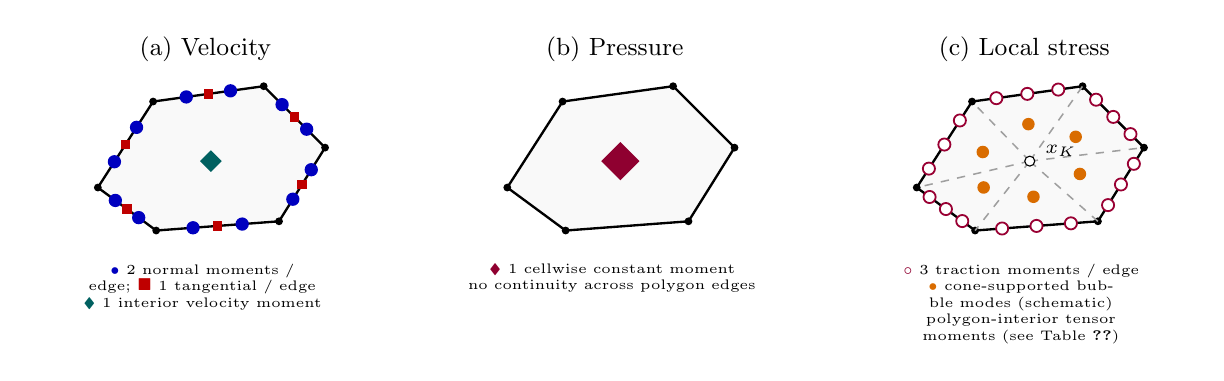
\begin{tikzpicture}[x=0.78cm,y=0.78cm,
  vertex/.style={circle,fill=black,inner sep=1.0pt},
  norm/.style={circle,fill=blue!75!black,inner sep=1.7pt},
  tang/.style={rectangle,fill=red!75!black,minimum size=3.4pt,inner sep=0pt},
  interior/.style={diamond,fill=teal!75!black,inner sep=2.0pt},
  traction/.style={circle,draw=purple!80!black,fill=white,line width=.65pt,inner sep=1.55pt},
  bubble/.style={circle,fill=orange!85!black,inner sep=1.6pt}]
\foreach \shift/\lab in {0/{(a) Velocity},5.2/{(b) Pressure},10.4/{(c) Local stress}} {
 \begin{scope}[xshift=\shift cm]
  \coordinate (A) at (0.3,0.7); \coordinate (B) at (1.2,2.1);
  \coordinate (C) at (3.0,2.35); \coordinate (D) at (4.0,1.35);
  \coordinate (E) at (3.25,0.15); \coordinate (F) at (1.25,0.0);
  \coordinate (O) at (2.14,1.13);
  \fill[gray!5] (A)--(B)--(C)--(D)--(E)--(F)--cycle;
  \draw[line width=.85pt] (A)--(B)--(C)--(D)--(E)--(F)--cycle;
  \foreach \v in {A,B,C,D,E,F} \node[vertex] at (\v) {};
  \node[font=\small] at (2.05,2.95) {\lab};
 \end{scope}
}
% Panel coordinates are re-established locally to avoid cross-panel references.
\begin{scope}
\coordinate (A) at (0.3,0.7); \coordinate (B) at (1.2,2.1);
\coordinate (C) at (3.0,2.35); \coordinate (D) at (4.0,1.35);
\coordinate (E) at (3.25,0.15); \coordinate (F) at (1.25,0.0);
\coordinate (O) at (2.14,1.13);
\foreach \u/\v in {A/B,B/C,C/D,D/E,E/F,F/A} {
 \path (\u)--(\v) coordinate[pos=.30] (mone) coordinate[pos=.70] (mtwo);
 \node[norm] at (mone) {}; \node[norm] at (mtwo) {};
 \path (\u)--(\v) coordinate[pos=.5] (mid);
 \node[tang] at (mid) {};
}
\node[interior] at (O) {};
\end{scope}
\begin{scope}[xshift=5.2cm]
\coordinate (O) at (2.14,1.13);
\node[interior,fill=purple!75!black,inner sep=3.5pt] at (O) {};
\end{scope}
\begin{scope}[xshift=10.4cm]
\coordinate (A) at (0.3,0.7); \coordinate (B) at (1.2,2.1);
\coordinate (C) at (3.0,2.35); \coordinate (D) at (4.0,1.35);
\coordinate (E) at (3.25,0.15); \coordinate (F) at (1.25,0.0);
\coordinate (O) at (2.14,1.13);
\foreach \v in {A,B,C,D,E,F} \draw[dashed,gray!75,line width=.55pt] (O)--(\v);
\filldraw[fill=white,draw=black] (O) circle (1.8pt);
\node[font=\scriptsize,anchor=west] at (2.24,1.30) {$x_K$};
\foreach \u/\v in {A/B,B/C,C/D,D/E,E/F,F/A} {
  \path (\u)--(\v) coordinate[pos=.22] (mone) coordinate[pos=.50] (mtwo) coordinate[pos=.78] (mthree);
  \node[traction] at (mone) {}; \node[traction] at (mtwo) {}; \node[traction] at (mthree) {};
  \path (O)--($(\u)!.5!(\v)$) coordinate[pos=.55] (ib);
  \node[bubble] at (ib) {};
}
\end{scope}
% compact panel legends, centered beneath the respective polygons
\node[align=center,font=\tiny,text width=4.2cm,anchor=north] at (2.0,-.38)
 {\textcolor{blue!75!black}{$\bullet$} 2 normal moments / edge; 
  \textcolor{red!75!black}{$\blacksquare$} 1 tangential / edge\\
  \textcolor{teal!75!black}{$\blacklozenge$} 1 interior velocity moment};
\node[align=center,font=\tiny,text width=4.2cm,anchor=north] at (8.67,-.38)
 {$\textcolor{purple!75!black}{\blacklozenge}$ 1 cellwise constant moment\\
  no continuity across polygon edges};
\node[align=center,font=\tiny,text width=4.2cm,anchor=north] at (15.33,-.38)
 {\textcolor{purple!75!black}{$\circ$} 3 traction moments / edge\\
  \textcolor{orange!85!black}{$\bullet$} cone-supported bubble modes (schematic)\\
  polygon-interior tensor moments (see Table~\ref{tab:k1-dof-count})};
\end{tikzpicture}%
}
\par\smallskip
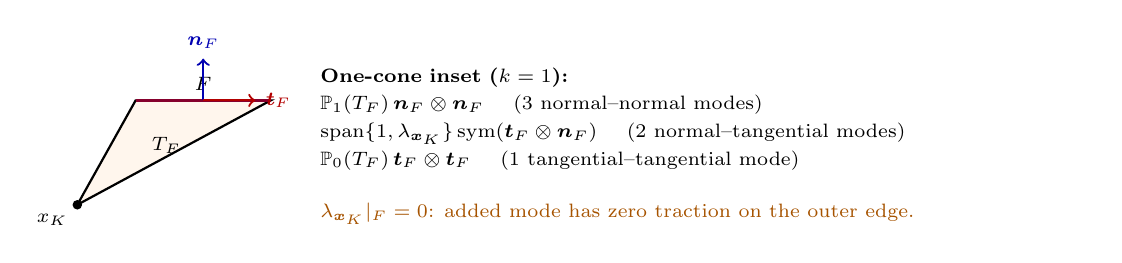
\begin{tikzpicture}[x=0.78cm,y=0.78cm,baseline=(current bounding box.center)]
  % One cone, with its outer primal edge and local tensor decomposition.
  \coordinate (X) at (0.1,0.15);
  \coordinate (L) at (1.05,1.85);
  \coordinate (R) at (3.25,1.85);
  \fill[orange!7] (X)--(L)--(R)--cycle;
  \draw[thick] (X)--(L)--(R)--cycle;
  \draw[line width=1.1pt,purple!70!black] (L)--(R);
  \filldraw[black] (X) circle (1.5pt);
  \node[below left,font=\scriptsize] at (X) {$x_K$};
  \node[above,font=\scriptsize] at ($(L)!.5!(R)$) {$F$};
  \node[font=\scriptsize] at (1.55,1.12) {$T_F$};
  \coordinate (M) at (2.15,1.85);
  \draw[->,blue!70!black,thick] (M)--++(0,0.68)
    node[above,font=\scriptsize] {$\boldsymbol n_F$};
  \draw[->,red!70!black,thick] (M)--++(0.85,0)
    node[right,font=\scriptsize] {$\boldsymbol t_F$};
  \node[anchor=west,font=\scriptsize,align=left,text width=9.7cm]
    at (3.9,1.55) {\textbf{One-cone inset ($k=1$):}\\[2pt]
    $\mathbb P_1(T_F)\,\boldsymbol n_F\otimes\boldsymbol n_F$
    \quad (3 normal--normal modes)\\[2pt]
    $\operatorname{span}\{1,\lambda_{\boldsymbol x_K}\}
       \operatorname{sym}(\boldsymbol t_F\otimes\boldsymbol n_F)$
    \quad (2 normal--tangential modes)\\[2pt]
    $\mathbb P_0(T_F)\,\boldsymbol t_F\otimes\boldsymbol t_F$
    \quad (1 tangential--tangential mode)};
  \node[anchor=west,font=\scriptsize,text=orange!65!black]
    at (3.9,0.0) {$\lambda_{\boldsymbol x_K}|_F=0$:
    added mode has zero traction on the outer edge.};
\end{tikzpicture}
\caption{Degrees of freedom and local reconstruction for $k=1$ on a hexagonal polygon $K$.
(a) The $H(\operatorname{div})$ velocity has two normal moments per edge and one interior
moment; the separate tangential trace has one moment per edge.
(b) The pressure has one cellwise constant moment.
(c) The enriched symmetric-tensor space is broken over the six cones
$T_F=\operatorname{conv}(x_K,F)$, where $x_K$ is the centroid. Each outer edge
has three local traction moments (two normal and one tangential). The orange symbols
indicate cone-supported bubble modes schematically, not individual degrees of freedom.
The inset displays the six local tensor modes on one cone, including the added normal--tangential bubble. The remaining interior tensor degrees of freedom are the three constant symmetric-tensor
moments and $\dim\mathcal Z_K=3N_K-3$ kernel moments, where $N_K$ is the number of edges.
Stress traction is not constrained to be continuous across radial cone interfaces or
between adjacent polygons, and the stress reconstruction adds no globally coupled unknowns.}
\label{fig:k1-dofs}
\end{figure}

\begin{table}[t]
\centering
\caption{Local degrees of freedom for $k=1$ on a polygon $K$ with
$N_K$ edges. The enriched symmetric-stress space has six local
coefficients per cone, but introduces no globally coupled stress unknowns.}
\label{tab:k1-dof-count}
\begin{tabular}{@{}llrr@{}}
\toprule
Variable & DoF family & General $N_K$ & $N_K=6$ \\
\midrule
Velocity & Edge normal moments & $2N_K$ & 12 \\
         & Edge tangential moments & $N_K$ & 6 \\
         & Interior Type III moment & $1$ & 1 \\
\cmidrule(lr){2-4}
         & Total & $3N_K+1$ & 19 \\
\midrule
Pressure & Interior constant moment & $1$ & 1 \\
\midrule
Stress & Outer-edge traction moments & $3N_K$ & 18 \\
       & Interior constant tensor moments & $3$ & 3 \\
       & Interior kernel moments ($\mathcal Z_K$) & $3N_K-3$ & 15 \\
\cmidrule(lr){2-4}
       & Total (local) & $6N_K$ & 36 \\
\bottomrule
\end{tabular}
\end{table}

\begin{remark}[Cost of the lowest-order enrichment]
For $k=1$, the original local symmetric-tensor space has five
polynomial coefficients per cone, whereas the enriched space
\eqref{eq:sigma1-enriched} has six. Thus the dimension of the
polygon-local stress space increases from $5N_K$ to $6N_K$,
with precisely one additional normal--tangential bubble mode
on each cone $T_F$. Since this mode has zero traction on the
outer edge $F$, the number of outer-edge stress traction moments
remains $3N_K$. The enrichment changes neither the velocity nor
the pressure degrees of freedom and introduces no globally
coupled stress unknowns. Moreover, because the tensor space is
broken across cones, its $L^2$ mass matrix is block diagonal
with respect to the cone subdivision: for $k=1$, the cone blocks
increase only from size $5\times5$ to $6\times6$.
\end{remark}

\begin{lemma}[Stable local lifting]\label{lem:stable-local-lifting}
Assume Assumption~\ref{bubbleassumption}.  Given
$\boldsymbol g_K\in\mathbb P_{k-1}(K;\mathbb S)$ and face data
$\boldsymbol r_F\in V_k(F)$, there is a unique
$\boldsymbol\sigma_K\in\Sigma_h^{-1}(K)$ whose polynomial moments equal
those of $\boldsymbol g_K$, whose traction moments equal those of
$\boldsymbol r_F$, and whose $\mathcal Z_K$ moments vanish. Moreover,
\begin{equation}\label{eq:stable-local-lifting}
\|\boldsymbol\sigma_K\|_K\lesssim
\|\boldsymbol g_K\|_K+
\sum_{F\subset\partial K}h_K^{1/2}\|\boldsymbol r_F\|_F .
\end{equation}
\end{lemma}
\begin{proof}
We construct the lifting in two stages, to exhibit the uniform
constant. Decompose each prescribed face vector as
$\boldsymbol r_F=r_F^n\boldsymbol n_F+\boldsymbol r_F^t$.
Extend its polynomial normal and tangential components from $F$ to
$T_F$ by keeping them constant on lines normal to $F$; denote these
extensions by $\widehat r_F^n$ and $\widehat{\boldsymbol r}_F^t$.
By the definition of $\Sigma_k(T_F)$, the tensor
\[
 \boldsymbol\sigma^{\rm tr}|_{T_F}
 =\widehat r_F^n\boldsymbol n_F\otimes\boldsymbol n_F
 +2\sym(\boldsymbol n_F\otimes
 \widehat{\boldsymbol r}_F^t)
\]
belongs to the local stress space and has exactly the prescribed
traction $\boldsymbol r_F$ on the base face $F$. The other cones
are independently treated in the same way. Fixed-degree polynomial
scaling on the uniformly regular cones yields
\begin{equation}\label{eq:trace-lift-bound}
 \|\boldsymbol\sigma^{\rm tr}\|_K
 \lesssim
 \Bigl(\sum_{F\subset\partial K}h_K\|\boldsymbol r_F\|_F^2
 \Bigr)^{1/2}.
\end{equation}

Let $P_{\mathcal Z_K}$ denote the $L^2(K)$-orthogonal projector onto
$\mathcal Z_K=\ker\mathcal M_K$ and define
$\boldsymbol\sigma^0=\boldsymbol\sigma^{\rm tr}
 -P_{\mathcal Z_K}\boldsymbol\sigma^{\rm tr}$.
Elements of $\mathcal Z_K$ are traction-free bubbles, so this
subtraction leaves all prescribed face moments unchanged.
Furthermore $\boldsymbol\sigma^0\perp\mathcal Z_K$ and
$\|\boldsymbol\sigma^0\|_K\le2\|\boldsymbol\sigma^{\rm tr}\|_K$.

The moment residual on $Q_K=\mathbb P_{k-1}(K;\mathbb S)$ is the
linear functional
\[
 L(\boldsymbol q)=(\boldsymbol g_K,\boldsymbol q)_K
 -(\boldsymbol\sigma^0,\boldsymbol q)_K,
 \qquad \boldsymbol q\in Q_K.
\]
Its dual $L^2$ norm is bounded by
$\|L\|_{Q_K^*}\le\|\boldsymbol g_K\|_K+
\|\boldsymbol\sigma^0\|_K$.
The intrinsic inf--sup condition is equivalent to the existence of a
unique $\boldsymbol\sigma^b\in\mathcal E_K$ for which
\[
 (\boldsymbol\sigma^b,\boldsymbol q)_K=L(\boldsymbol q)
 \quad(\boldsymbol q\in Q_K),\qquad
 \|\boldsymbol\sigma^b\|_K\le\beta_*^{-1}\|L\|_{Q_K^*}.
\]
Finally set $\boldsymbol\sigma_K=\boldsymbol\sigma^0+
\boldsymbol\sigma^b$. Its face tractions are $\boldsymbol r_F$;
its $Q_K$ moments equal those of $\boldsymbol g_K$; and both terms
are orthogonal to $\mathcal Z_K$. The estimates above imply
\[
 \|\boldsymbol\sigma_K\|_K
 \le (1+\beta_*^{-1})\|\boldsymbol\sigma^0\|_K
 +\beta_*^{-1}\|\boldsymbol g_K\|_K
 \lesssim \|\boldsymbol g_K\|_K+
 \Bigl(\sum_F h_K\|\boldsymbol r_F\|_F^2\Bigr)^{1/2},
\]
which is stronger than \eqref{eq:stable-local-lifting}.
Existence follows from this construction and uniqueness from
Lemma~\ref{lemma_DOF}.
\end{proof}

Let
\[
\Sigma_h^{-1} = \{\boldsymbol{\sigma} \in L^2(\Omega;\mathbb{S}) : \boldsymbol{\sigma}|_T \in \Sigma_k(T), T \in \mathcal{T}_h\}.
\]

\subsection{Weak strain}
For any \(\boldsymbol{v} = \{ \boldsymbol{v}^{\operatorname{div}}, \boldsymbol{v}^t \} \in \boldsymbol{V}_h\),
we define \(\varepsilon^w_h(\boldsymbol{v}) \in \Sigma_h^{-1}\) satisfying \( \varepsilon^w_h(\boldsymbol{v})|_K=\varepsilon_K^w(\boldsymbol{v})\) and
\begin{equation}\label{equ:weakstrain1}
\begin{aligned}
(\varepsilon_K^w(\boldsymbol v),\boldsymbol\sigma)_K
={}&(\varepsilon(\boldsymbol\Pi_K^o\boldsymbol v^{\operatorname{div}}),\boldsymbol\sigma)_K\\
&+\langle(\boldsymbol v^{\operatorname{div}}-
 \boldsymbol\Pi_K^o\boldsymbol v^{\operatorname{div}})\cdot\boldsymbol n,
 (\boldsymbol\sigma\boldsymbol n)\cdot\boldsymbol n\rangle_{\partial K}\\
&+\langle\boldsymbol v^t-\Pi_F\boldsymbol\Pi_K^o\boldsymbol v^{\operatorname{div}},
 \Pi_F(\boldsymbol\sigma\boldsymbol n)\rangle_{\partial K}
\end{aligned}
\end{equation}
for all $\boldsymbol\sigma\in\Sigma_h^{-1}(K)$, with $\Pi_F$ applied facewise.
Since $\boldsymbol\sigma$ is discontinuous inside $K$, integration by
parts must include the internal jumps of $\boldsymbol\sigma\boldsymbol n$.
Dropping these terms does not give an equivalent definition.

The normal and tangential boundary jumps are
\[
\begin{aligned}
\mathcal J_{\partial K}^{\boldsymbol n}(\boldsymbol v)
&:=((\boldsymbol v^{\operatorname{div}}-
\boldsymbol\Pi_K^o\boldsymbol v^{\operatorname{div}})\cdot\boldsymbol n)\boldsymbol n,\\
\mathcal J_{\partial K}^{\boldsymbol\tau}(\boldsymbol v)
&:=\boldsymbol v^t-\Pi_F\boldsymbol\Pi_K^o\boldsymbol v^{\operatorname{div}}.
\end{aligned}
\]
Their sum is $\mathcal J_{\partial K}(\boldsymbol v):=
\mathcal J_{\partial K}^{\boldsymbol n}(\boldsymbol v)+
\mathcal J_{\partial K}^{\boldsymbol\tau}(\boldsymbol v)$.

 On the face \(F \subset \partial K\), we define \((\boldsymbol{\Pi}_{\partial K}^t \boldsymbol{v})|_F \in \boldsymbol{V}_F\) as
\[
\int_F \boldsymbol{\Pi}_{\partial K}^t \boldsymbol{v} \cdot \boldsymbol{q}\,\mathrm ds = \int_F \boldsymbol{v}|_K \cdot \boldsymbol{q}\,\mathrm ds \quad \forall \boldsymbol{q} \in \boldsymbol{V}_F.
\]
Define the notation \(\boldsymbol{\Pi}_{\partial K}\) as
\[
\boldsymbol{\Pi}_{\partial K} \boldsymbol{v} := (\boldsymbol{v} \cdot \boldsymbol{n})\boldsymbol{n} + \boldsymbol{\Pi}_{\partial K}^t \boldsymbol{v}.
\]

Since $\boldsymbol\sigma\boldsymbol n|_F\in V_k(F)$, \eqref{equ:weakstrain1} becomes
\[
(\varepsilon_K^w(\boldsymbol{v}), \boldsymbol{\sigma})_K = (\varepsilon(\boldsymbol{\Pi}_K^o \boldsymbol{v}^{\operatorname{div}}), \boldsymbol{\sigma})_K + \langle \boldsymbol{\Pi}_{\partial K} \mathcal{J}_{\partial K}(\boldsymbol{v}), \boldsymbol{\sigma}\boldsymbol{n} \rangle_{\partial K}.
\]


For $\boldsymbol v_h\in\boldsymbol V_h$, define the mesh-dependent seminorm
\[
\|\boldsymbol{v}_h\|_{1,h}^2 := \sum_{K \in \mathcal{K}_h} \|\boldsymbol{v}_h\|_{1,h,K}^2,
\]
where the seminorm on each element is defined as
\[
\|\boldsymbol{v}_h\|_{1,h,K}^2 := \|\varepsilon (\boldsymbol{\Pi}_K^o \boldsymbol{v}_h^{\operatorname{div}})\|_K^2 + h_K^{-1}\|\boldsymbol{\Pi}_{\partial K}\mathcal{J}_{\partial K}(\boldsymbol{v}_h)\|_{\partial K}^2.
\]


\begin{lemma}\label{lem:norm}
The mesh-dependent quantity
\(
\|\boldsymbol{v}_h\|_{1,h}
\)
defines a norm on the virtual element space \(\boldsymbol{V}_h\).
\end{lemma}

\begin{proof}
If $\|\boldsymbol v_h\|_{1,h}=0$, then on each $K$,
$\boldsymbol\Pi_K^o\boldsymbol v_h^{\operatorname{div}}=\boldsymbol r_K
\in\mathbf{RM}(K)$, and
\[
\boldsymbol v_h^{\operatorname{div}}\cdot\boldsymbol n
=\boldsymbol r_K\cdot\boldsymbol n,
\qquad
\boldsymbol v_h^t=\Pi_F\boldsymbol r_K\quad\text{on each }F\subset\partial K.
\]
The second identity uses $\Pi_F\boldsymbol r_K\in\mathbf{RM}(F)$.
The normal component of $\boldsymbol v_h^{\operatorname{div}}$ and the
single-valued tangential field $\boldsymbol v_h^t$ show that neighboring
rigid motions agree on their common face. A rigid motion that vanishes on
a face is zero, so connectedness gives one global rigid motion $\boldsymbol r$.
The boundary conditions give both $\boldsymbol r\cdot\boldsymbol n=0$ and
$\Pi_F\boldsymbol r=0$ on boundary faces. Hence $\boldsymbol r=0$.
The normal face moments and all polynomial volume moments of
$\boldsymbol v_h^{\operatorname{div}}$ now vanish. Unisolvence of
$\boldsymbol V_K$ gives $\boldsymbol v_h^{\operatorname{div}}=0$,
and the tangential identity gives $\boldsymbol v_h^t=0$.
\end{proof}

We also need control of the full jump. For
$\boldsymbol w=\boldsymbol\Pi_K^o\boldsymbol v_h^{\operatorname{div}}$,
Korn's inequality modulo rigid motions gives a $\boldsymbol r_K\in\mathbf{RM}(K)$
such that
\[
h_K^{-1}\|\boldsymbol w-\boldsymbol r_K\|_K
+\|\nabla(\boldsymbol w-\boldsymbol r_K)\|_K
\lesssim\|\varepsilon(\boldsymbol w)\|_K.
\]
Since $\boldsymbol\Pi_{\partial K}^t$ reproduces $\Pi_F\boldsymbol r_K$,
the trace inequality yields
\[
h_K^{-1/2}\|\Pi_F\boldsymbol w-
\boldsymbol\Pi_{\partial K}^t\boldsymbol w\|_{\partial K}
\lesssim\|\varepsilon(\boldsymbol w)\|_K.
\]
The normal part of the jump is unchanged by $\boldsymbol\Pi_{\partial K}$.
The unprojected tangential part has the same norm as the difference above. Thus
\begin{equation}\label{eq:fulljump}
h_K^{-1/2}\|\mathcal J_{\partial K}(\boldsymbol v_h)\|_{\partial K}
\lesssim\|\boldsymbol v_h\|_{1,h,K}.
\end{equation}
The jump of $\boldsymbol w$ across a primal face is the difference of its
two full boundary jumps; on a boundary face, $\boldsymbol w$ is minus its
full boundary jump. Applying the broken Korn inequality \cite{Brenner2004}
on the simplicial refinement therefore gives the global equivalence
\begin{equation}\label{eq:globalKorn}
\|\boldsymbol v_h\|_{1,h}^2\simeq
\sum_{K\in\mathcal K_h}\left(
\|\nabla\boldsymbol\Pi_K^o\boldsymbol v_h^{\operatorname{div}}\|_K^2
+h_K^{-1}\|\boldsymbol\Pi_{\partial K}\mathcal J_{\partial K}(\boldsymbol v_h)\|_{\partial K}^2
\right).
\end{equation}
This equivalence is global; it does not hold on an individual element.

\begin{lemma} \label{lem:discinf-sup}
We have the discrete inf-sup condition
\begin{equation}\label{eq:discinfsup}
\|\boldsymbol{v}\|_{1,h}\lesssim \sup_{0\ne\boldsymbol{\sigma}_h\in\Sigma_h^{-1}}
\frac{\sum_{K\in\mathcal{K}_h}(\varepsilon_K^w(\boldsymbol{v}), \boldsymbol{\sigma}_h)_K}{\|\boldsymbol{\sigma}_h\|_{0,h}}\quad\forall~\boldsymbol{v}\in\boldsymbol V_h.
\end{equation}
\end{lemma}
\begin{proof}
Here $\|\boldsymbol\sigma\|_{0,h}^2:=\sum_K\|\boldsymbol\sigma\|_K^2$.
For fixed $\boldsymbol v\in\boldsymbol V_h$, use Lemma~\ref{lemma_DOF}
to choose $\boldsymbol\sigma|_K\in\Sigma_h^{-1}(K)$ with
\[
\begin{aligned}
(\boldsymbol\sigma,\boldsymbol\tau)_K
&=(\varepsilon(\boldsymbol\Pi_K^o\boldsymbol v^{\operatorname{div}}),\boldsymbol\tau)_K
&&\forall\boldsymbol\tau\in\mathbb P_{k-1}(K;\mathbb S),\\
\langle\boldsymbol\sigma\boldsymbol n,\boldsymbol q\rangle_F
&=\langle h_K^{-1}\boldsymbol\Pi_{\partial K}\mathcal J_{\partial K}(\boldsymbol v),\boldsymbol q\rangle_F
&&\forall\boldsymbol q\in V_k(F),\ F\subset\partial K,
\end{aligned}
\]
and with the moments \eqref{SigmaKDoFs2} set to zero.
Face moments are prescribed separately on each element side, using its
outward normal. Testing with the polynomial strain and projected jump gives
\[
\sum_K(\varepsilon_K^w(\boldsymbol v),\boldsymbol\sigma)_K
=\|\boldsymbol v\|_{1,h}^2.
\]
Applying the stable local lifting, Lemma~\ref{lem:stable-local-lifting}, with the prescribed polynomial and traction moments gives
\[
\begin{aligned}
\|\boldsymbol\sigma\|_K
&\lesssim\|\varepsilon(\boldsymbol\Pi_K^o\boldsymbol v^{\operatorname{div}})\|_K
+h_K^{-1/2}\|\boldsymbol\Pi_{\partial K}\mathcal J_{\partial K}(\boldsymbol v)\|_{\partial K},\\
\|\boldsymbol\sigma\|_{0,h}&\lesssim\|\boldsymbol v\|_{1,h}.
\end{aligned}
\]
Substitute this tensor into the supremum in \eqref{eq:discinfsup}.
The result follows for $\boldsymbol v\ne0$; the zero case is immediate.
\end{proof}



\begin{lemma}\label{lem:coercive-strain}
For every $\boldsymbol v_h\in\boldsymbol V_h$,
\[
\|\boldsymbol v_h\|_{1,h}\lesssim\|\varepsilon_h^w(\boldsymbol v_h)\|.
\]
\end{lemma}
\begin{proof}
Apply Lemma~\ref{lem:discinf-sup} and the Cauchy--Schwarz inequality.
\end{proof}

\section{Numerical scheme}\label{sec:scheme}
Let
\[
S_h:=\{q_h\in L_0^2(\Omega):q_h|_K\in\mathbb P_{k-1}(K)
\text{ for all }K\in\mathcal K_h\}.
\]
The discrete formulation of \eqref{eq:stokes} seeks
$\boldsymbol u_h=\{\boldsymbol u_h^{\operatorname{div}},\boldsymbol u_h^t\}
\in\boldsymbol V_h$ and $p_h\in S_h$ such that
\begin{equation}\label{eq:scheme}
\left\{\begin{aligned}
a_h(\boldsymbol u_h,\boldsymbol v_h)+b(\boldsymbol v_h,p_h)
&=(\boldsymbol f,\boldsymbol\Pi_h^o\boldsymbol v_h^{\operatorname{div}})
&&\forall\boldsymbol v_h\in\boldsymbol V_h,\\
b(\boldsymbol u_h,q_h)&=0&&\forall q_h\in S_h,
\end{aligned}\right.
\end{equation}
where
\[
a_h(\boldsymbol u_h,\boldsymbol v_h):=
(\varepsilon_h^w(\boldsymbol u_h),\varepsilon_h^w(\boldsymbol v_h)),
\qquad
b(\boldsymbol v_h,p_h):=-(\operatorname{div}\boldsymbol v_h^{\operatorname{div}},p_h).
\]


\begin{remark}[Gradient forces and pressure robustness]
\label{rem:pressure-gradient} Although the discrete velocity is
exactly divergence-free, this alone does not guarantee full
pressure robustness, since the elementwise $L^2$ projection
$\boldsymbol\Pi_h^o\boldsymbol v_h^{\operatorname{div}}$ used in
the load term of \eqref{eq:scheme} is generally neither
divergence-free nor $H(\operatorname{div})$-conforming; see
\cite{FrerichsMerdon2022} for a related discussion and a
divergence-preserving reconstruction.

Nevertheless, the method is invariant under polynomial gradient
forces. More precisely, let $\phi\in H^1(\Omega)$ satisfy
$\nabla\phi|_K\in\mathbb P_k(K;\mathbb R^2)$ for every
$K\in\mathcal T_h$. Then
\[
\begin{aligned}
(\nabla\phi,
 \boldsymbol\Pi_h^o\boldsymbol v_h^{\operatorname{div}})
&=(\nabla\phi,\boldsymbol v_h^{\operatorname{div}})\\
&=-(\phi,\operatorname{div}
          \boldsymbol v_h^{\operatorname{div}})\\
&=b(\boldsymbol v_h,Q_h\phi),
\end{aligned}
\]
where $Q_h$ denotes the $L^2$ projection onto $S_h$. Here we have
used polynomial orthogonality, normal conformity, and the
homogeneous normal boundary condition. Consequently, replacing
$\boldsymbol f$ by $\boldsymbol f+\nabla\phi$ leaves the discrete
velocity unchanged and shifts the discrete pressure from $p_h$ to
$p_h+Q_h\phi$.

%For general gradient forces, this invariance need not hold, and
%full pressure robustness is not established for the present
%formulation.
\end{remark}


\subsection{Local viscous stress and equivalent formulation}
The viscosity is normalized so that the physical viscous stress is
$\boldsymbol\tau=\varepsilon(\boldsymbol u)$ and the total Cauchy stress is
$\boldsymbol\sigma=\boldsymbol\tau-p\boldsymbol I$.
For each element define the strongly symmetric discrete viscous stress
$\boldsymbol\tau_h|_K\in\Sigma_h^{-1}(K)$ by
\begin{equation}\label{eq:stress-local}
(\boldsymbol\tau_h,\boldsymbol\eta_h)_K
=(\varepsilon_K^w(\boldsymbol u_h),\boldsymbol\eta_h)_K
\qquad\forall\boldsymbol\eta_h\in\Sigma_h^{-1}(K).
\end{equation}
The corresponding local mixed representation of
\eqref{eq:scheme} is: find
$(\boldsymbol\tau_h,\boldsymbol u_h,p_h)$ such that
\begin{equation}\label{eq:stress-mixed}
\left\{\begin{aligned}
(\boldsymbol\tau_h-\varepsilon_K^w(\boldsymbol u_h),\boldsymbol\eta_h)_K&=0
&&\forall\boldsymbol\eta_h\in\Sigma_h^{-1}(K),\ K\in\mathcal K_h,\\
\sum_K(\boldsymbol\tau_h,\varepsilon_K^w(\boldsymbol v_h))_K
+b(\boldsymbol v_h,p_h)&=(\boldsymbol f,\boldsymbol\Pi_h^o\boldsymbol v_h^{\operatorname{div}})
&&\forall\boldsymbol v_h\in\boldsymbol V_h,\\
b(\boldsymbol u_h,q_h)&=0&&\forall q_h\in S_h.
\end{aligned}\right.
\end{equation}
The first equation yields
$\boldsymbol\tau_h=\varepsilon_h^w(\boldsymbol u_h)$;
substitution gives precisely \eqref{eq:scheme}. Thus the stress is
computed locally and adds no globally coupled unknowns.
The following proposition records three structural properties of the
reconstructed stress. The tensor
$\boldsymbol\sigma_h=\boldsymbol\tau_h-p_h\boldsymbol I$ is symmetric
on each cone, but neither traction continuity nor a strong local
momentum balance is asserted.


\begin{proposition}[Symmetry, energy identity, and bubble orthogonality of the reconstructed stress]
\label{prop:stress-properties}
Let $\boldsymbol\tau_h=\varepsilon_h^w(\boldsymbol u_h)$ and set
$\boldsymbol G_K=\varepsilon(\boldsymbol\Pi_K^o
\boldsymbol u_h^{\operatorname{div}})$. Then
\begin{equation}\label{eq:stress-properties}
\begin{aligned}
\boldsymbol\tau_h|_K&\in\Sigma_h^{-1}(K),\\
a_h(\boldsymbol u_h,\boldsymbol u_h)
 &=\sum_{K\in\mathcal K_h}\|\boldsymbol\tau_h\|_{0,K}^2,\\
(\boldsymbol\tau_h-\boldsymbol G_K,\boldsymbol\eta_h)_K
 &=0\qquad\forall\boldsymbol\eta_h\in \mathbb B_k(\div,K;\mathbb S).
\end{aligned}
\end{equation}
Here $\mathbb B_k(\div,K;\mathbb S)$ is defined in \eqref{eq:bubblespace}.
\end{proposition}
\begin{proof}
The first assertion follows from the definition of the local
symmetric-tensor space. The second follows from the definition of
$a_h$ and $\boldsymbol\tau_h=\varepsilon_h^w(\boldsymbol u_h)$.
For $\boldsymbol\eta_h\in \mathbb B_k(\div,K;\mathbb S)$, its normal traction vanishes on
$\partial K$. Testing \eqref{equ:weakstrain1} with
$\boldsymbol\eta_h$ therefore eliminates both boundary terms and gives
$(\varepsilon_K^w(\boldsymbol u_h),\boldsymbol\eta_h)_K
=(\boldsymbol G_K,\boldsymbol\eta_h)_K$, as claimed.
\end{proof}
The reconstructed total stress
$\boldsymbol\sigma_h=\boldsymbol\tau_h-p_h\boldsymbol I$ is
strongly symmetric elementwise. The reconstruction does not, in
general, impose continuity of $\boldsymbol\sigma_h\boldsymbol n$
across element interfaces or strong elementwise momentum equilibrium.

\begin{lemma}
For every
\(
\boldsymbol{v}_h=\{\boldsymbol{v}_h^{\operatorname{div}},\boldsymbol{v}_h^t\}\in \boldsymbol{V}_h,
\)
there holds
\[
\|\varepsilon_h^w(\boldsymbol{v}_h)\|^2
\lesssim
\|\boldsymbol{v}_h\|_{1,h}^2.
\]
\end{lemma}

\begin{proof}
Set $\boldsymbol\sigma=\varepsilon_K^w(\boldsymbol v_h)$ in
\eqref{equ:weakstrain1}. The Cauchy--Schwarz and polynomial trace inequalities give
\[
\begin{aligned}
\|\varepsilon_K^w(\boldsymbol v_h)\|_K^2
\lesssim\Bigl(&\|\varepsilon(\boldsymbol\Pi_K^o\boldsymbol v_h^{\operatorname{div}})\|_K\\
&+h_K^{-1/2}\|\boldsymbol\Pi_{\partial K}\mathcal J_{\partial K}(\boldsymbol v_h)\|_{\partial K}\Bigr)
\|\varepsilon_K^w(\boldsymbol v_h)\|_K.
\end{aligned}
\]
Divide by the strain norm when it is nonzero, square, and sum over $K$.
\end{proof}


\begin{lemma}\label{lem:10}
For $\boldsymbol u_h,\boldsymbol v_h\in\boldsymbol V_h$,
\begin{align*}
|a_h(\boldsymbol{u}_h, \boldsymbol{v}_h)| &\lesssim \|\boldsymbol{u}_h\|_{1,h} \|\boldsymbol{v}_h\|_{1,h}, \\
a_h(\boldsymbol{u}_h, \boldsymbol{u}_h) &\gtrsim  \|\boldsymbol{u}_h\|_{1,h}^2.
\end{align*}
\end{lemma}




\begin{lemma}\label{lem:11}
For $\boldsymbol v_h\in\boldsymbol V_h$ and $q_h\in S_h$,
\[
|b(\boldsymbol v_h,q_h)|\lesssim\|\boldsymbol v_h\|_{1,h}\|q_h\|.
\]
\end{lemma}
\begin{proof}
Write $\boldsymbol w=\boldsymbol\Pi_K^o\boldsymbol v_h^{\operatorname{div}}$.
For $q\in\mathbb P_{k-1}(K)$, the volume projection and integration by parts give
\[
(\operatorname{div}\boldsymbol v_h^{\operatorname{div}},q)_K
=(\operatorname{div}\boldsymbol w,q)_K
+\langle\mathcal J_{\partial K}^{\boldsymbol n}(\boldsymbol v_h)\cdot\boldsymbol n,q\rangle_{\partial K}.
\]
Use $q=\operatorname{div}\boldsymbol v_h^{\operatorname{div}}$, the polynomial
trace inequality, and $|\operatorname{div}\boldsymbol w|\leq
\sqrt d\,|\varepsilon(\boldsymbol w)|$. This gives
$\|\operatorname{div}\boldsymbol v_h^{\operatorname{div}}\|_K
\lesssim\|\boldsymbol v_h\|_{1,h,K}$.
Sum over $K$ and apply the Cauchy--Schwarz inequality.
\end{proof}

\begin{lemma}\label{lem:12}
For every $p_h\in S_h$, there is a $\boldsymbol v_h\in\boldsymbol V_h$ with
\[
\operatorname{div}\boldsymbol v_h^{\operatorname{div}}=p_h,
\qquad\|\boldsymbol v_h\|_{1,h}\lesssim\|p_h\|.
\]
\end{lemma}

\subsection{Interpolation}
For $\boldsymbol v\in\boldsymbol H^1(K)$, define
$\boldsymbol I_K^{\operatorname{div}}\boldsymbol v\in\boldsymbol V_K$
by matching its Type I--III DoFs with those of $\boldsymbol v$.
Integration by parts with $q\in\mathbb P_{k-1}(K)$ gives the commuting identity
\begin{equation}\label{eq:commuting}
\operatorname{div}\boldsymbol I_K^{\operatorname{div}}\boldsymbol v
=Q_h(\operatorname{div}\boldsymbol v)|_K,
\end{equation}
where $Q_h$ is the elementwise $L^2$ projection onto $\mathbb P_{k-1}$;
for mean-zero functions its range is $S_h$.
The interpolant reproduces $\mathbb P_k(K;\mathbb R^d)$.
Scaled stability of its DoFs gives
\begin{equation}\label{eq:Istability}
\|\boldsymbol I_K^{\operatorname{div}}\boldsymbol v\|_K
\lesssim\|\boldsymbol v\|_K+h_K|\boldsymbol v|_{1,K}.
\end{equation}
Indeed, the scaled face moments are bounded by
$h_K^{1/2}\|\boldsymbol v\cdot\boldsymbol n\|_{\partial K}$,
and the normalized volume moments by $\|\boldsymbol v\|_K$.
The trace inequality and uniform norm equivalence for the unisolvent DoFs
prove \eqref{eq:Istability}. These arguments are the usual face-VEM
interpolation estimates; see \cite{BBMR2016,BMM2022} for the underlying
spaces and related stability results. Subtracting a degree-$k$ polynomial
approximant in \eqref{eq:Istability} yields
\begin{equation}\label{eq:Iapprox}
\|\boldsymbol v-\boldsymbol I_K^{\operatorname{div}}\boldsymbol v\|_K
\lesssim h_K^{k+1}|\boldsymbol v|_{k+1,K}.
\end{equation}

\begin{proof}[Proof of Lemma~\ref{lem:12}]
The continuous divergence right inverse \cite{BBF2013} provides
$\boldsymbol v\in\boldsymbol H_0^1(\Omega)$ with
$\operatorname{div}\boldsymbol v=p_h$ and
$|\boldsymbol v|_1\lesssim\|p_h\|$.
Set $\boldsymbol v_h^{\operatorname{div}}|_K=
\boldsymbol I_K^{\operatorname{div}}\boldsymbol v$ and
$\boldsymbol v_h^t|_F=\boldsymbol\Pi_{\partial K}^t\boldsymbol v$.
The traces are single-valued and zero on the boundary, and
\eqref{eq:commuting} gives the required divergence.
Let $\boldsymbol w=\boldsymbol\Pi_K^o\boldsymbol I_K^{\operatorname{div}}\boldsymbol v$.
Subtracting the mean of $\boldsymbol v$ in \eqref{eq:Istability}, and using
polynomial inverse estimates, gives
\[
\|\nabla\boldsymbol w\|_K\lesssim|\boldsymbol v|_{1,K},
\qquad
\|\boldsymbol v-\boldsymbol w\|_K\lesssim h_K|\boldsymbol v|_{1,K}.
\]
The normal interpolant trace is the face $L^2$ projection of
$\boldsymbol v\cdot\boldsymbol n$. Thus both parts of the projected boundary
jump are bounded by $\|\boldsymbol v-\boldsymbol w\|_{\partial K}$.
The trace inequality now gives
$\|\boldsymbol v_h\|_{1,h,K}\lesssim|\boldsymbol v|_{1,K}$.
Sum over $K$ to conclude.
\end{proof}
Since $b$ has a minus sign, use the negative of this lifting to obtain
\begin{equation}\label{eq:pressure-infsup}
\|q_h\|\lesssim\sup_{0\ne\boldsymbol v_h\in\boldsymbol V_h}
\frac{|b(\boldsymbol v_h,q_h)|}{\|\boldsymbol v_h\|_{1,h}}
\qquad(q_h\in S_h).
\end{equation}
Together with Lemmas~\ref{lem:10} and \ref{lem:11}, this proves that
\eqref{eq:scheme} has a unique solution \cite{BBF2013}.
Also, $\operatorname{div}\boldsymbol u_h^{\operatorname{div}}\in S_h$;
testing the second equation with this divergence shows that it vanishes
on every element.

\subsection{Error equations}
Assume $(\boldsymbol u,p)\in
(\boldsymbol H^{k+1}(\Omega)\cap\boldsymbol H_0^1(\Omega))\times
(H^k(\Omega)\cap L_0^2(\Omega))$ solves \eqref{eq:stokes}.
Set
\[
\boldsymbol u_I^{\operatorname{div}}|_K=\boldsymbol I_K^{\operatorname{div}}\boldsymbol u,
\qquad \boldsymbol u_I^t|_F=\boldsymbol\Pi_{\partial K}^t\boldsymbol u,
\qquad p_I=Q_hp.
\]
For later use, \eqref{eq:Iapprox}, polynomial approximation, and inverse
estimates imply
\begin{equation}\label{eq:projected-approx}
\begin{aligned}
&\|\boldsymbol u-\boldsymbol\Pi_K^o\boldsymbol I_K^{\operatorname{div}}\boldsymbol u\|_K
+h_K|\boldsymbol u-\boldsymbol\Pi_K^o\boldsymbol I_K^{\operatorname{div}}\boldsymbol u|_{1,K}\\
&\quad+h_K^{1/2}\|\boldsymbol u-\boldsymbol\Pi_K^o\boldsymbol I_K^{\operatorname{div}}\boldsymbol u\|_{\partial K}
\lesssim h_K^{k+1}|\boldsymbol u|_{k+1,K}.
\end{aligned}
\end{equation}
To see this, subtract a degree-$k$ polynomial approximant and bound the
remaining polynomial by its $L^2$ norm using inverse and trace estimates.
The same argument applied to the strain gives
\begin{equation}\label{eq:strain-approx}
\begin{aligned}
&\|\varepsilon(\boldsymbol u)-\varepsilon(\boldsymbol\Pi_K^o
\boldsymbol I_K^{\operatorname{div}}\boldsymbol u)\|_K\\
&\quad+h_K^{1/2}\|\varepsilon(\boldsymbol u)-\varepsilon(\boldsymbol\Pi_K^o
\boldsymbol I_K^{\operatorname{div}}\boldsymbol u)\|_{\partial K}
\lesssim h_K^k|\boldsymbol u|_{k+1,K}.
\end{aligned}
\end{equation}
Since the normal interpolant trace and the tangential interpolant are face
projections, \eqref{eq:projected-approx} also gives
\begin{equation}\label{eq:interpolant-jump}
h_K^{-1/2}\|\boldsymbol\Pi_{\partial K}\mathcal J_{\partial K}(\boldsymbol u_I)\|_{\partial K}
\lesssim h_K^k|\boldsymbol u|_{k+1,K}.
\end{equation}

Set $e_h=\boldsymbol u_h-\boldsymbol u_I$ and $\xi_h=p_h-p_I$.
The error equation is
Write $\boldsymbol E_K=\varepsilon(\boldsymbol u)-
\varepsilon(\boldsymbol\Pi_K^o\boldsymbol u_I^{\operatorname{div}})$ and
$\boldsymbol w_K=\boldsymbol v_h^{\operatorname{div}}-
\boldsymbol\Pi_K^o\boldsymbol v_h^{\operatorname{div}}$.
The error equation is
\begin{equation}\label{eq:erroreq}
\begin{aligned}
a_h(e_h,\boldsymbol v_h)+b(\boldsymbol v_h,\xi_h)
=\mathcal R(\boldsymbol v_h):=\sum_{K\in\mathcal K_h}\bigl[&
(\boldsymbol E_K,\varepsilon(\boldsymbol\Pi_K^o\boldsymbol v_h^{\operatorname{div}}))_K\\
&+\langle\mathcal J_{\partial K}(\boldsymbol v_h),\boldsymbol E_K\boldsymbol n\rangle_{\partial K}
+\langle Q_hp-p,\boldsymbol w_K\cdot\boldsymbol n\rangle_{\partial K}\\
&-\langle\boldsymbol\Pi_{\partial K}\mathcal J_{\partial K}(\boldsymbol u_I),
\varepsilon_K^w(\boldsymbol v_h)\boldsymbol n\rangle_{\partial K}\bigr].
\end{aligned}
\end{equation}
for all $\boldsymbol v_h\in\boldsymbol V_h$.
To derive it, test \eqref{eq:stokes} with
$\boldsymbol\Pi_K^o\boldsymbol v_h^{\operatorname{div}}$, integrate by parts,
and sum over $K$. The exact traction paired with
$(\boldsymbol v_h^{\operatorname{div}}\cdot\boldsymbol n)\boldsymbol n+\boldsymbol v_h^t$
cancels on interior faces and vanishes on the boundary.
For the pressure terms, the volume projection preserves moments against
$\nabla(Q_hp)$, and
\[
(\operatorname{div}\boldsymbol\Pi_K^o\boldsymbol v_h^{\operatorname{div}},p-Q_hp)_K=0.
\]
For the strain terms, use \eqref{equ:weakstrain1} twice and recall that
$\varepsilon(\boldsymbol\Pi_K^o\boldsymbol u_I^{\operatorname{div}})
\in\mathbb P_{k-1}(K;\mathbb S)\subset\Sigma_h^{-1}(K)$.
Its normal trace belongs to $V_k(F)$, so it pairs equally with the projected
and full jumps.
By \eqref{eq:commuting}, $\operatorname{div}\boldsymbol u_I^{\operatorname{div}}=0$.
Hence
\begin{equation}\label{eq:divergenceerror}
b(e_h,q_h)=0\qquad\forall q_h\in S_h.
\end{equation}

We estimate the four terms in \eqref{eq:erroreq} in order.
The volume strain term is bounded by \eqref{eq:strain-approx} and the norm
of $\boldsymbol v_h$. The boundary strain term uses the same approximation
estimate and the full-jump bound \eqref{eq:fulljump}.
For the pressure term, the local projection estimate is
\[
h_K^{1/2}\|p-Q_hp\|_{\partial K}\lesssim h_K^k|p|_{k,K};
\]
its other factor is the normal part of the jump, which the discrete norm
controls directly. Finally, the polynomial trace inequality and the weak-strain
upper bound give
\[
\begin{aligned}
&|\langle\boldsymbol\Pi_{\partial K}\mathcal J_{\partial K}(\boldsymbol u_I),
\varepsilon_K^w(\boldsymbol v_h)\boldsymbol n\rangle_{\partial K}|\\
&\qquad\lesssim h_K^{-1/2}
\|\boldsymbol\Pi_{\partial K}\mathcal J_{\partial K}(\boldsymbol u_I)\|_{\partial K}
\|\boldsymbol v_h\|_{1,h,K}.
\end{aligned}
\]
Use \eqref{eq:interpolant-jump}, then sum the estimates over $K$.
The Cauchy--Schwarz inequality yields
\begin{equation}\label{eq:residual-bound}
|\mathcal R(\boldsymbol v_h)|\lesssim
h^k(\|\boldsymbol u\|_{k+1}+\|p\|_k)\|\boldsymbol v_h\|_{1,h}.
\end{equation}

\subsection{Error estimates}
Taking $\boldsymbol v_h=e_h$ in \eqref{eq:erroreq} and
$q_h=\xi_h$ in \eqref{eq:divergenceerror}, coercivity gives
\[
\|e_h\|_{1,h}^2\lesssim a_h(e_h,e_h)=\mathcal R(e_h).
\]
Therefore, \eqref{eq:residual-bound} implies
\[
\|e_h\|_{1,h}\lesssim h^k(\|\boldsymbol u\|_{k+1}+\|p\|_k).
\]
For the pressure, \eqref{eq:pressure-infsup} and \eqref{eq:erroreq} give
\[
\begin{aligned}
\|\xi_h\|&\lesssim\sup_{0\ne\boldsymbol v_h\in\boldsymbol V_h}
\frac{|\mathcal R(\boldsymbol v_h)-a_h(e_h,\boldsymbol v_h)|}{\|\boldsymbol v_h\|_{1,h}}\\
&\lesssim\|e_h\|_{1,h}+h^k(\|\boldsymbol u\|_{k+1}+\|p\|_k).
\end{aligned}
\]
Thus $\|\xi_h\|$ has the same bound.

In the velocity error norm, identify the smooth velocity with the pair
$\{\boldsymbol u,\boldsymbol\Pi_{\partial K}^t\boldsymbol u\}$, and use the same
norm formula with the $L^2$ volume projector.
Polynomial approximation and \eqref{eq:Iapprox} give
$\|\boldsymbol u-\boldsymbol u_I\|_{1,h}\lesssim h^k\|\boldsymbol u\|_{k+1}$.
The triangle inequality and $\|p-Q_hp\|\lesssim h^k\|p\|_k$ then yield
\begin{equation}\label{eq:final-error}
\|\boldsymbol u-\boldsymbol u_h\|_{1,h}+\|p-p_h\|
\lesssim h^k(\|\boldsymbol u\|_{k+1}+\|p\|_k).
\end{equation}


\begin{theorem}[Error estimate for the reconstructed viscous stress]
\label{thm:stress-error}
Under the assumptions of the preceding velocity--pressure error estimate,
let $\boldsymbol\tau=\varepsilon(\boldsymbol u)$ and
$\boldsymbol\tau_h=\varepsilon_h^w(\boldsymbol u_h)$.
Then
\begin{equation}\label{eq:stress-error}
\color{blue}
\|\boldsymbol\tau-\boldsymbol\tau_h\|_{0,\Omega}
\lesssim h^k\bigl(\|\boldsymbol u\|_{k+1,\Omega}
                  +\|p\|_{k,\Omega}\bigr).
\end{equation}
\end{theorem}
\begin{proof}
Let $\boldsymbol u_I$ be the velocity interpolant defined above, and
write $\boldsymbol G_K=\varepsilon(\boldsymbol\Pi_K^o
\boldsymbol u_I^{\operatorname{div}})$.
Since $\mathbb P_{k-1}(K;\mathbb S)\subset\Sigma_h^{-1}(K)$,
$\boldsymbol G_K$ belongs to the local stress space. The defining
identity \eqref{equ:weakstrain1} therefore implies
\[
\bigl(\varepsilon_K^w(\boldsymbol u_I)-\boldsymbol G_K,
\boldsymbol\eta_h\bigr)_K
=\bigl\langle\boldsymbol\Pi_{\partial K}
\mathcal J_{\partial K}(\boldsymbol u_I),
\boldsymbol\eta_h\boldsymbol n\bigr\rangle_{\partial K}
\qquad(\boldsymbol\eta_h\in\Sigma_h^{-1}(K)).
\]
Taking $\boldsymbol\eta_h=\varepsilon_K^w(\boldsymbol u_I)-
\boldsymbol G_K$ and using the polynomial inverse trace inequality
on the local stress space gives
\begin{equation}\label{eq:stress-correction-bound}
\|\varepsilon_K^w(\boldsymbol u_I)-\boldsymbol G_K\|_{0,K}
\lesssim h_K^{-1/2}\|\boldsymbol\Pi_{\partial K}
\mathcal J_{\partial K}(\boldsymbol u_I)\|_{0,\partial K}
\lesssim h_K^k|\boldsymbol u|_{k+1,K},
\end{equation}
where the last inequality is \eqref{eq:interpolant-jump}.
Together with \eqref{eq:strain-approx}, this yields
\begin{equation}\label{eq:stress-interpolation}
\|\boldsymbol\tau-\varepsilon_h^w(\boldsymbol u_I)\|_{0,\Omega}
\lesssim h^k\|\boldsymbol u\|_{k+1,\Omega}.
\end{equation}
Finally, linearity of the weak strain, its upper stability bound,
and the discrete velocity estimate proved above imply
\[
\begin{aligned}
\|\boldsymbol\tau-\boldsymbol\tau_h\|_{0,\Omega}
&\le\|\boldsymbol\tau-\varepsilon_h^w(\boldsymbol u_I)\|_{0,\Omega}
 +\|\varepsilon_h^w(\boldsymbol u_I-\boldsymbol u_h)\|_{0,\Omega}\\
&\lesssim h^k\|\boldsymbol u\|_{k+1,\Omega}
 +\|\boldsymbol u_I-\boldsymbol u_h\|_{1,h}\\
&\lesssim h^k\bigl(\|\boldsymbol u\|_{k+1,\Omega}
 +\|p\|_{k,\Omega}\bigr),
\end{aligned}
\]
as claimed.
\end{proof}

% !TEX root = SEVEM_Stokes.tex
\section{Numerical results}\label{sec:numerics}

\AI{For $k=1$, the velocity uses $\boldsymbol V_h$ and the pressure is
piecewise constant on the primal mesh $\mathcal K_h$.
The coefficient of the symmetric strain in \eqref{eq:stokes} is one,
which corresponds to $2\nu=1$ in the usual viscosity convention.
The weak strain \eqref{equ:weakstrain1} has the equivalent form
\[
(\varepsilon_K^w(\boldsymbol v),\boldsymbol\sigma)_K
=-(\boldsymbol v^{\operatorname{div}},\operatorname{div}_{w,K}\boldsymbol\sigma)_K
+\langle\boldsymbol v^{\operatorname{div}}\cdot\boldsymbol n,
 (\boldsymbol\sigma\boldsymbol n)\cdot\boldsymbol n\rangle_{\partial K}
+\langle\boldsymbol v^t,\Pi_F(\boldsymbol\sigma\boldsymbol n)\rangle_{\partial K},
\]
where $\boldsymbol\sigma\in\Sigma_h^{-1}(K)$ with $k=1$, and
$\operatorname{div}_{w,K}\boldsymbol\sigma\in\mathbb P_1(K;\mathbb R^d)$ satisfies
\[
(\operatorname{div}_{w,K}\boldsymbol\sigma,\boldsymbol q)_K
=-(\boldsymbol\sigma,\nabla\boldsymbol q)_K
+\langle\boldsymbol\sigma\boldsymbol n,\boldsymbol q\rangle_{\partial K}
\qquad\forall\boldsymbol q\in\mathbb P_1(K;\mathbb R^d).
\]
This definition includes the internal stress jumps through integration by
parts on the cones. Its equivalence follows from the volume projection
and the symmetry of $\boldsymbol\sigma$.}

The reported \texttt{sincosdata} test is posed on the unit square.
Tables~\ref{tab:poly}--\ref{tab:rect} give the supplied results.
\AI{The energy error is $\|\boldsymbol u_I-\boldsymbol u_h\|_{A_h}
:=a_h(\boldsymbol u_I-\boldsymbol u_h,\boldsymbol u_I-\boldsymbol u_h)^{1/2}$.
The energy and total pressure errors approach first-order convergence on
these meshes. Faster convergence in some other columns is an empirical
observation; it is not proved by \eqref{eq:final-error}.}

\AI{\begin{remark}[Numerical data to confirm]
The supplied files do not specify the exact velocity, pressure, force,
boundary data, viscosity used in the computations, or the definitions of
$\|\cdot\|_{0,h}$ and the reported maximum norms.
The implemented strain space must also be checked against
\eqref{eq:strainspace}; the original numerical description used a different
index. The table values are retained pending these checks.
The rectangular meshes do not satisfy Assumption~\ref{meshassumption}:
their face-tangential tensors span only diagonal symmetric matrices.
Table~\ref{tab:rect} therefore reports a test outside the proved mesh class.
The three mesh figure files were not supplied.
\end{remark}}

% ===== Table 1 =====
\begin{table}[htbp]
  \centering \footnotesize
  \caption{Results on polygonal meshes obtained from a triangle-mesh dual.}\label{tab:poly}
  \setlength{\tabcolsep}{3pt}\resizebox{\textwidth}{!}{\begin{tabular}{cccccccc}
    \toprule
    DoFs & $h$ & $\|\boldsymbol u_I-\boldsymbol u_h\|_{A_h}$ & $\|\boldsymbol u_I-\boldsymbol u_h\|_{0,h}$ & $\|\boldsymbol u_I-\boldsymbol u_h\|_{\infty}$ & $\|p_I-p_h\|$ & $\|p-p_h\|$ & $\|p_I-p_h\|_{\text{max}}$ \\
    \midrule
    314   & 1.43e-01 & 8.767e-01 & 2.588e-02 & 7.996e-02 & 2.071e-01 & 2.454e-01 & 5.002e-01 \\
    978   & 7.78e-02 & 4.012e-01 & 9.135e-03 & 2.645e-02 & 6.612e-02 & 1.007e-01 & 1.870e-01 \\
    3362  & 4.12e-02 & 1.884e-01 & 2.712e-03 & 7.111e-03 & 1.936e-02 & 4.463e-02 & 7.481e-02 \\
    12354 & 2.13e-02 & 9.119e-02 & 7.279e-04 & 1.817e-03 & 5.869e-03 & 2.145e-02 & 3.068e-02 \\
    47234 & 1.08e-02 & 4.490e-02 & 1.875e-04 & 4.573e-04 & 1.874e-03 & 1.061e-02 & 1.335e-02 \\
    \bottomrule
  \end{tabular}}
\end{table}

% ===== Table 2 =====
\begin{table}[htbp]
  \centering\footnotesize
  \caption{Results on triangular meshes.}\label{tab:tri}
  \setlength{\tabcolsep}{3pt}\resizebox{\textwidth}{!}{\begin{tabular}{cccccccc}
    \toprule
    DoFs & $h$ & $\|\boldsymbol u_I-\boldsymbol u_h\|_{A_h}$ & $\|\boldsymbol u_I-\boldsymbol u_h\|_{0,h}$ & $\|\boldsymbol u_I-\boldsymbol u_h\|_{\infty}$ & $\|p_I-p_h\|$ & $\|p-p_h\|$ & $\|p_I-p_h\|_{\text{max}}$ \\
    \midrule
    232   & 2.50e-01 & 4.289e-01 & 1.463e-02 & 3.022e-02 & 5.357e-01 & 5.509e-01 & 8.008e-01 \\
    880   & 1.25e-01 & 1.949e-01 & 2.959e-03 & 6.035e-03 & 2.867e-01 & 2.940e-01 & 4.262e-01 \\
    3424  & 6.25e-02 & 9.410e-02 & 6.990e-04 & 1.479e-03 & 1.450e-01 & 1.486e-01 & 2.115e-01 \\
    13504 & 3.12e-02 & 4.659e-02 & 1.727e-04 & 4.138e-04 & 7.265e-02 & 7.446e-02 & 1.045e-01 \\
    53632 & 1.56e-02 & 2.323e-02 & 4.308e-05 & 1.098e-04 & 3.634e-02 & 3.725e-02 & 5.187e-02 \\
    \bottomrule
  \end{tabular}}
\end{table}

% ===== Table 3 =====
\begin{table}[htbp]
  \centering\footnotesize
  \caption{Results on rectangular meshes, outside Assumption~\ref{meshassumption}.}\label{tab:rect}
  \setlength{\tabcolsep}{3pt}\resizebox{\textwidth}{!}{\begin{tabular}{cccccccc}
    \toprule
    DoFs & $h$ & $\|\boldsymbol u_I-\boldsymbol u_h\|_{A_h}$ & $\|\boldsymbol u_I-\boldsymbol u_h\|_{0,h}$ & $\|\boldsymbol u_I-\boldsymbol u_h\|_{\infty}$ & $\|p_I-p_h\|$ & $\|p-p_h\|$ & $\|p_I-p_h\|_{\text{max}}$ \\
    \midrule
    152    & 2.50e-01 & 6.193e-01 & 4.377e-02 & 7.423e-02 & 1.557e-02 & 1.574e-01 & 2.227e-02 \\
    560    & 1.25e-01 & 2.438e-01 & 1.277e-02 & 1.582e-02 & 9.016e-03 & 8.021e-02 & 1.778e-02 \\
    2144   & 6.25e-02 & 1.083e-01 & 3.348e-03 & 4.464e-03 & 2.688e-03 & 4.011e-02 & 6.658e-03 \\
    8384   & 3.12e-02 & 5.211e-02 & 8.477e-04 & 1.148e-03 & 6.957e-04 & 2.004e-02 & 1.943e-03 \\
    33152  & 1.56e-02 & 2.579e-02 & 2.126e-04 & 2.889e-04 & 1.752e-04 & 1.002e-02 & 5.205e-04 \\
    \bottomrule
  \end{tabular}}
\end{table}

% The figure is included only when all three supplied assets are available.
\IfFileExists{fig/poly.pdf}{%
  \IfFileExists{fig/tri.pdf}{%
    \IfFileExists{fig/rect.pdf}{%
      \begin{figure}[htbp]
      \centering
      \includegraphics[width=.31\textwidth]{fig/poly.pdf}\hfill
      \includegraphics[width=.31\textwidth]{fig/tri.pdf}\hfill
      \includegraphics[width=.31\textwidth]{fig/rect.pdf}
      \caption{Polygonal, triangular, and rectangular test meshes.}\label{fig:meshes}
      \end{figure}
    }{}%
  }{}%
}{}%



\clearpage
\begin{thebibliography}{12}
\bibitem{BBCMMR2013}
L. Beir\~ao da Veiga, F. Brezzi, A. Cangiani, G. Manzini, L. D. Marini, and A. Russo,
\emph{Basic principles of virtual element methods},
Math. Models Methods Appl. Sci., 23 (2013), pp. 199--214,
\url{https://doi.org/10.1142/S0218202512500492}.

\bibitem{BBMR2016}
L. Beir\~ao da Veiga, F. Brezzi, L. D. Marini, and A. Russo,
\emph{$H(\mathrm{div})$ and $H(\mathrm{curl})$-conforming virtual element methods},
Numer. Math., 133 (2016), pp. 303--332,
\url{https://doi.org/10.1007/s00211-015-0746-1}.

\bibitem{BMM2022}
L. Beir\~ao da Veiga, L. Mascotto, and J. Meng,
\emph{Interpolation and stability estimates for edge and face virtual elements of general order},
Math. Models Methods Appl. Sci., 32 (2022), pp. 1589--1631,
\url{https://doi.org/10.1142/S0218202522500373}.

\bibitem{BBF2013}
D. Boffi, F. Brezzi, and M. Fortin,
\emph{Mixed Finite Element Methods and Applications},
Springer Series in Computational Mathematics, vol. 44, Springer, Heidelberg, 2013,
\url{https://doi.org/10.1007/978-3-642-36519-5}.

\bibitem{Brenner2004}
S. C. Brenner,
\emph{Korn's inequalities for piecewise $H^1$ vector fields},
Math. Comp., 73 (2004), pp. 1067--1087,
\url{https://doi.org/10.1090/S0025-5718-03-01579-5}.

\bibitem{ChenWang2019}
L. Chen and F. Wang,
\emph{A divergence free weak virtual element method for the Stokes problem on polytopal meshes},
J. Sci. Comput., 78 (2019), pp. 864--886,
\url{https://doi.org/10.1007/s10915-018-0796-5}.

\bibitem{ChenHuangWei2024}
C. Chen, X. Huang, and H. Wei,
\emph{Virtual element methods without extrinsic stabilization},
SIAM J. Numer. Anal., 62 (2024), pp. 567--591,
\url{https://doi.org/10.1137/22M1504196}.

\bibitem{FrerichsMerdon2022}
D. Frerichs and C. Merdon,
\emph{Divergence-preserving reconstructions on polygons and a really
pressure-robust virtual element method for the Stokes problem},
IMA J. Numer. Anal., 42 (2022), pp. 597--619,
\url{https://doi.org/10.1093/imanum/draa073}.

\bibitem{MuYeZhang2021}
L. Mu, X. Ye, and S. Zhang,
\emph{A stabilizer-free, pressure-robust, and superconvergence weak Galerkin
finite element method for the Stokes equations on polytopal mesh},
SIAM J. Sci. Comput., 43 (2021), pp. A2614--A2637,
\url{https://doi.org/10.1137/20M1380405}.
\end{thebibliography}

\end{document}
